\documentclass{article}
\usepackage[main,final,nonatbib]{neurips_2025}

\usepackage{iftex}
\ifPDFTeX
  \usepackage[utf8]{inputenc}
  \usepackage[T1]{fontenc}
\else
  \usepackage{fontspec}
  \IfFontExistsTF{TeX Gyre Termes}{\setmainfont{TeX Gyre Termes}}{\setmainfont{Liberation Serif}}
  \IfFontExistsTF{TeX Gyre Heros}{\setsansfont{TeX Gyre Heros}}{\setsansfont{Liberation Sans}}
  \IfFontExistsTF{Latin Modern Mono}{\setmonofont{Latin Modern Mono}}{\setmonofont{Liberation Mono}}
\fi
\usepackage{hyperref}
\usepackage{url}
\usepackage{booktabs}
\usepackage{graphicx}
\usepackage{amsmath}
\usepackage{amssymb}
\usepackage{microtype}
\usepackage{xcolor}
\usepackage{enumitem}
\usepackage{float}
\usepackage{placeins}
\usepackage{caption}

\title{DSAA2011 Covertype Project Report}

\author{%
  Zeyun DU, Zixiang QIN, Chunfeng GAO\\
  DSAA2011 Machine Learning Course Project\\
  \texttt{ZeyunDU\_covertype}
}

\begin{document}
\maketitle

\begin{abstract}
We study the UCI Covertype dataset, which contains 581,012 forest observations described by 54 cartographic variables and labeled with one of seven forest cover types. The workflow covers preprocessing, t-SNE visualization, two clustering algorithms, four supervised classifiers, cross-validation, probability calibration, feature analysis, and subgroup robustness. Unsupervised methods reveal broad terrain structure but align poorly with the ecological labels: the strongest ARI among the internally selected solutions is 0.103; switching to Gower distance with complete linkage raises the post-hoc ARI to 0.245, though absolute agreement remains low. In contrast, nonlinear ensembles model the labeled structure effectively. Random Forest obtains the strongest test performance, with 0.9076 accuracy, 0.9076 macro-F1, and 0.9923 macro one-vs-rest AUC.  We use stratified 5-fold cross-validation and bootstrap confidence intervals (1,000 resamples) to quantify the stability of these rankings; a paired McNemar test confirms systematic per-sample error-pattern differences ($p<0.001$), while bootstrap confidence intervals show the macro-F1 gap between the two best models is stable but practically negligible ($\Delta = 0.0094$).  Elevation is the most influential feature, while road, fire-point, hydrology, soil, and wilderness variables provide additional signal. Error and subgroup analyses show that Lodgepole Pine, Spruce/Fir, mid-elevation observations, and Cache la Poudre Wilderness remain comparatively difficult.
\end{abstract}

\section{Introduction}

Forest cover is shaped by interacting topographic, hydrological, and ecological conditions. Predicting cover type from cartographic measurements is therefore a useful multi-class learning problem: a successful model must capture nonlinear relations while remaining reliable for uncommon classes. The Covertype dataset \cite{blackard1998comparison,blackard1999comparative,uci} contains 581,012 observations of $30\times30$ meter forest patches from Roosevelt National Forest in Colorado. Its 54 predictors comprise 10 continuous terrain variables, four wilderness-area indicators, and 40 soil-type indicators. The response has seven classes: Spruce/Fir, Lodgepole Pine, Ponderosa Pine, Cottonwood/Willow, Aspen, Douglas-fir, and Krummholz.

Figure~\ref{fig:data_profile}a shows severe class imbalance. Lodgepole Pine and Spruce/Fir together account for 85.3\% of the data, whereas Cottonwood/Willow represents only 0.5\%. Accuracy alone could consequently conceal poor minority-class performance, so we emphasize macro-averaged precision, recall, F1, and one-vs-rest AUC. The standardized continuous-feature distributions in Figure~\ref{fig:data_profile}b also retain long tails and outliers, suggesting that linear decision boundaries may be restrictive even after scale differences are removed.

This report is organized as follows. Section~2 presents the mandatory tasks, including data preprocessing, t-SNE visualization and clustering analysis, model training with baseline classifiers, and confusion matrix evaluation. Section~3 discusses open-ended exploration, covering feature engineering, model selection, calibration, and robustness diagnostics. Section~4 concludes with a summary of key findings and insights.

\begin{figure}[tbp]
  \centering
  \begin{minipage}{0.48\linewidth}
    \centering
    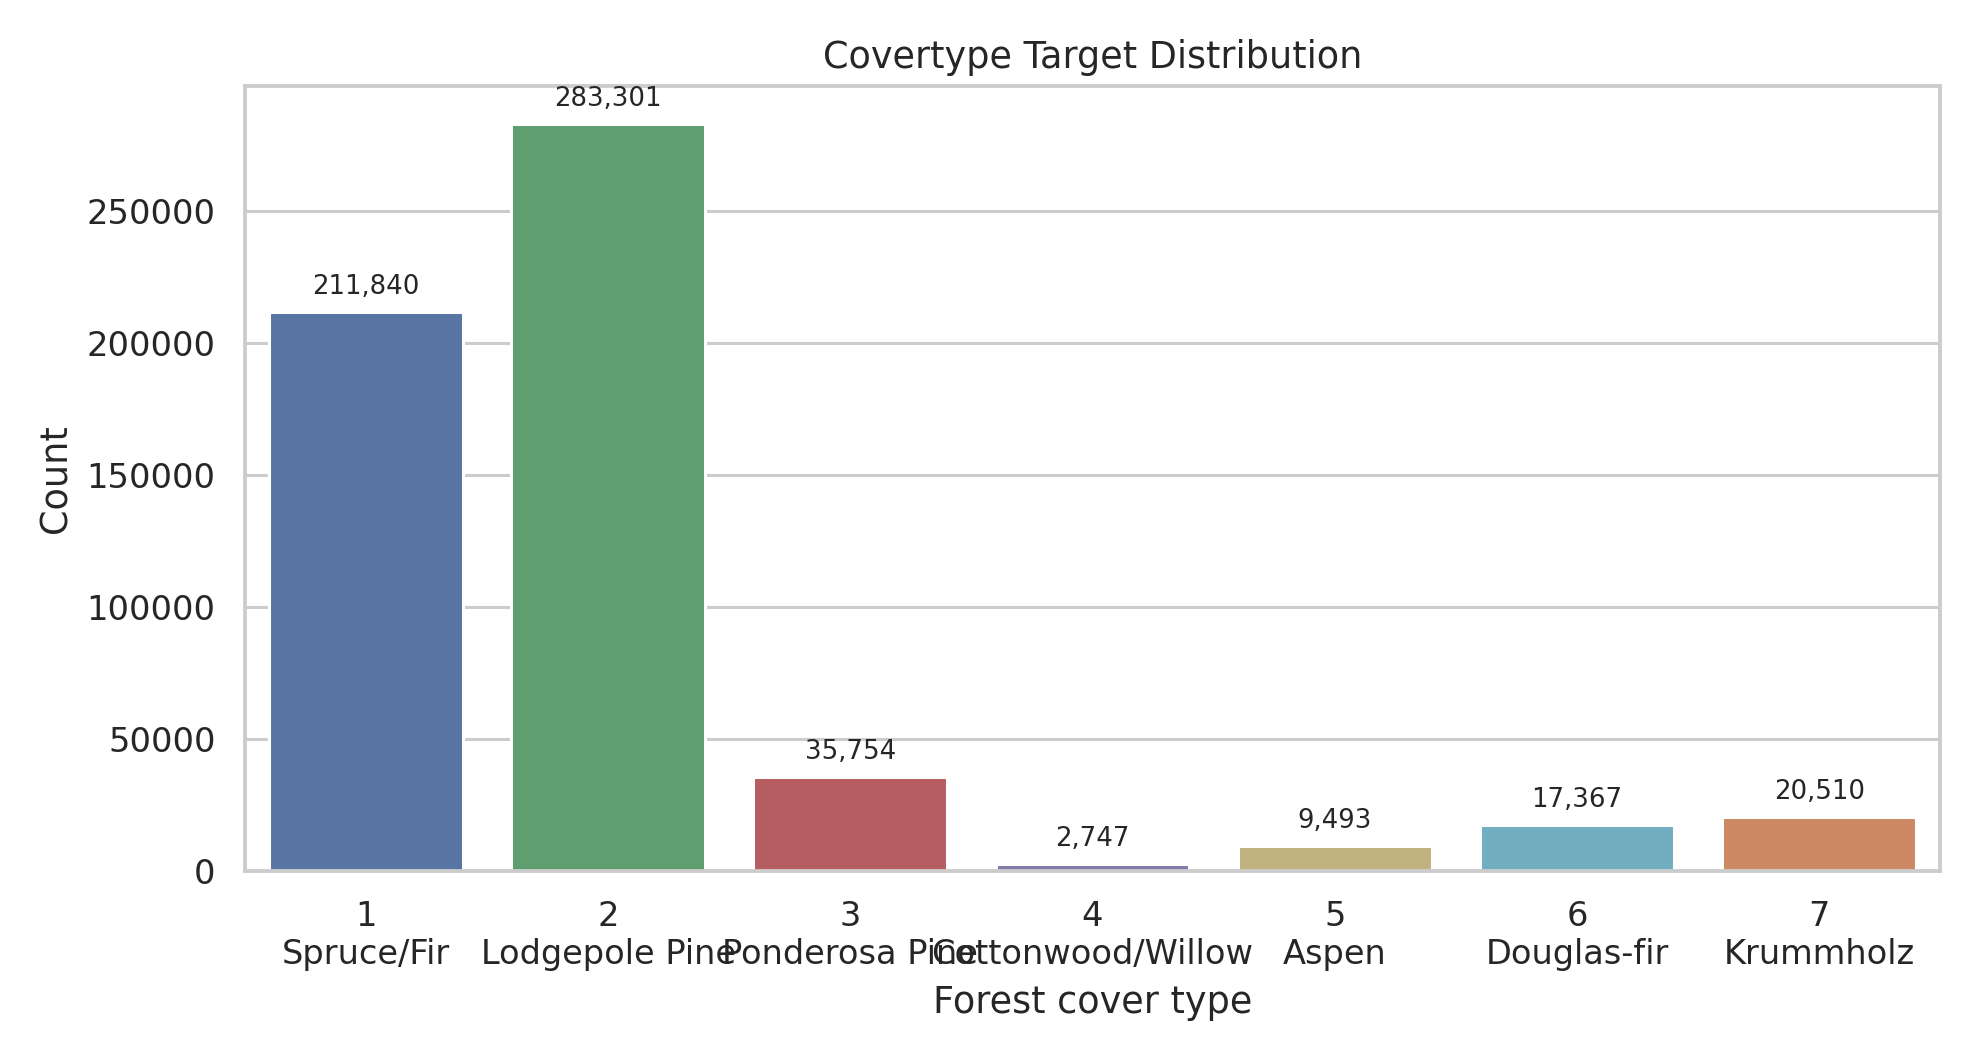
\includegraphics[width=\linewidth]{figures/target_distribution.png}\\[-0.4ex]
    \small (a) Cover-type distribution
  \end{minipage}\hfill
  \begin{minipage}{0.48\linewidth}
    \centering
    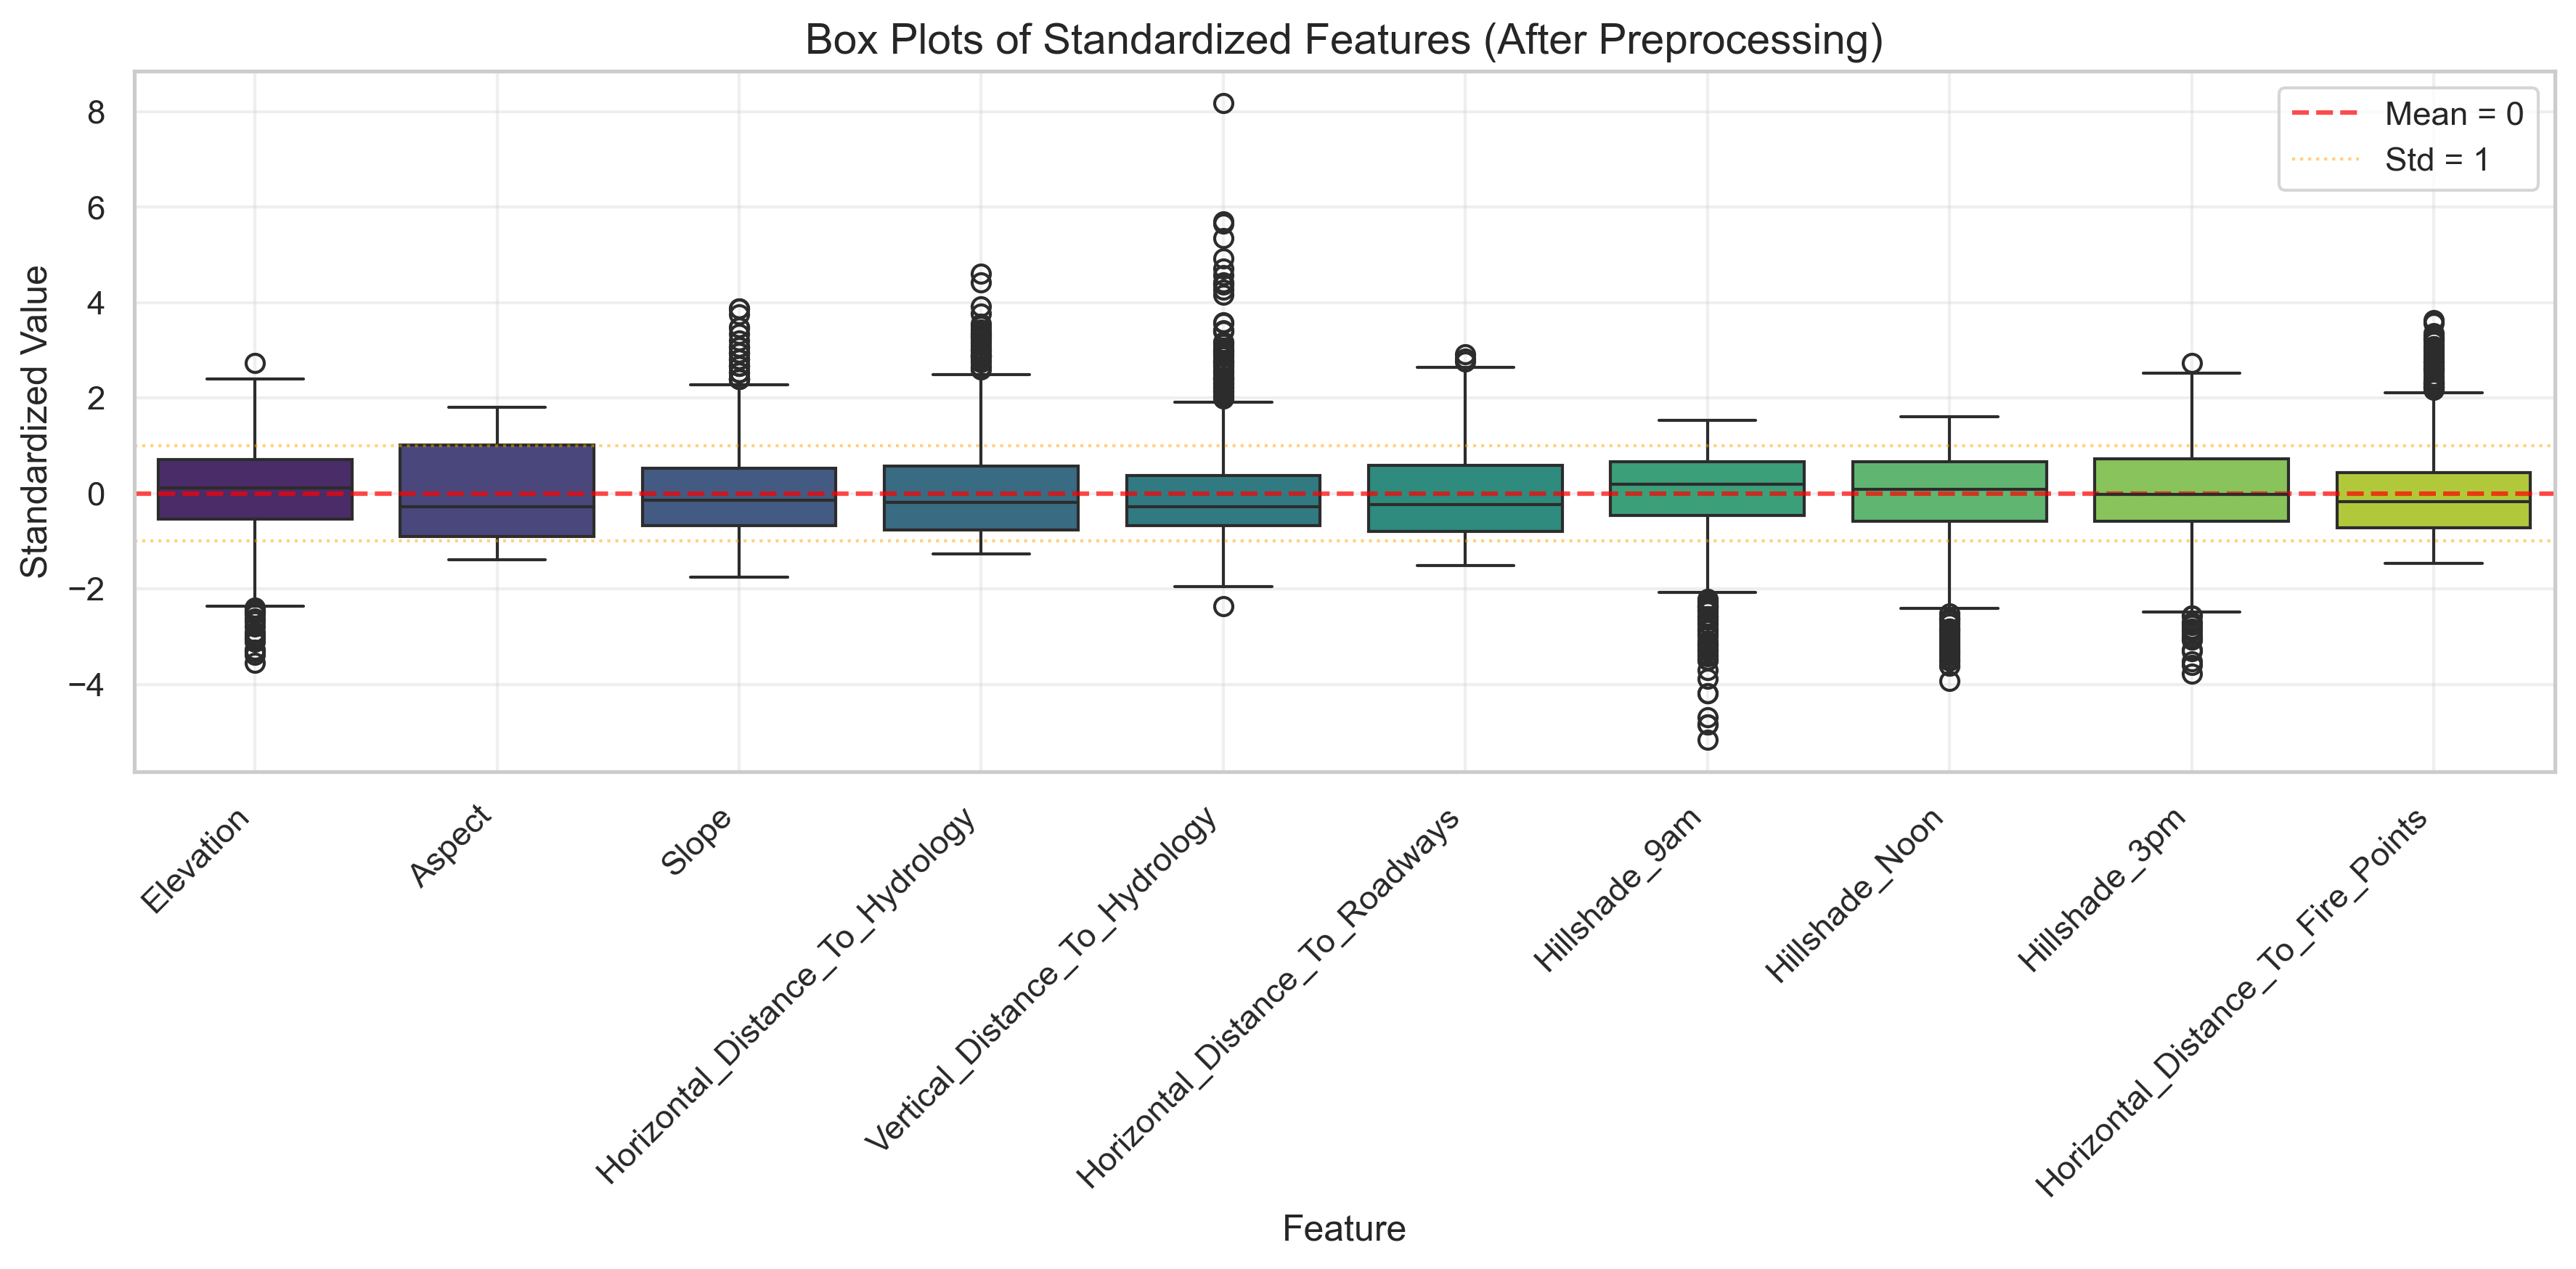
\includegraphics[width=\linewidth]{figures/boxplots_after.png}\\[-0.4ex]
    \small (b) Standardized continuous variables
  \end{minipage}
  \caption{Dataset profile. The response is dominated by classes 1 and 2, while standardized continuous variables remain heterogeneous and contain substantial tails.}
  \label{fig:data_profile}
\end{figure}

\FloatBarrier
\section{Mandatory Tasks}

\subsection{Data Preprocessing}

The raw UCI file is numeric and has no header. We assign the official feature names and verify the type and admissible range of every column. No missing values are present, so no observations or predictors are removed. The implementation places continuous and indicator variables in separate preprocessing branches: continuous variables would be median-imputed if needed and binary indicators would be mode-imputed. This design prevents a future missing value from breaking the pipeline and avoids treating indicator columns as continuous measurements.

For logistic regression, t-SNE, K-Means, and Ward clustering, each continuous predictor is standardized using
\begin{equation}
z=\frac{x-\mu}{\sigma},
\label{eq:standardization}
\end{equation}
where $\mu$ and $\sigma$ are estimated exclusively from the sub-sample used for each specific analysis (t-SNE: 5,999; clustering: 2,500--5,999; supervised: 68,565 training), not from the full 581,012-observation dataset. For the supervised pipeline, the StandardScaler is fitted on the 68,565-row training split only and applied via \texttt{transform} to the held-out 29,385 test observations, following the strict train/test separation protocol. Binary wilderness and soil indicators remain in $\{0,1\}$. Tree models receive the same predictors without requiring scale normalization. Stratification is used whenever a sample or train-test split is drawn, preserving rare classes such as Cottonwood/Willow. Finally, continuous columns are stored as \texttt{float32} and indicators as \texttt{uint8}; the resulting dataframe requires about 47.1 MB rather than the 244 MB estimated for an all-\texttt{int64} representation. The 44 binary features can additionally be stored in sparse CSR format for further memory savings, while HistGradientBoosting's histogram-based binning is inherently memory-efficient and requires no sparse input. The entire notebook executes within course-project laptop resources.

\subsection{t-SNE Visualization}

t-SNE \cite{tsne} is computationally expensive on more than half a million points, so we use a reproducible stratified sample of 5,999 observations. Continuous features are standardized and the 54-dimensional matrix is compressed to 50 principal components before t-SNE. PCA removes redundant directions and reduces computational cost, while stratification ensures that all seven labels remain visible. The embedding is obtained by minimizing
\begin{equation}
\text{KL}(P\|Q)=\sum_{i\neq j}p_{ij}\log\frac{p_{ij}}{q_{ij}},
\label{eq:tsne}
\end{equation}
where $p_{ij}$ and $q_{ij}$ describe pairwise neighborhood similarities in the high- and low-dimensional spaces. Thus, nearby observations are emphasized more strongly than global geometric distances.

The projection in Figure~\ref{fig:tsne} shows meaningful local organization but not seven clean islands. Krummholz and some Spruce/Fir observations occupy distinctive high-elevation regions, whereas Spruce/Fir and Lodgepole Pine overlap over much of the map. Rare classes form local pockets instead of globally isolated groups. Because t-SNE preserves local neighborhoods rather than global distances, the plot is not evidence of a specific number of clusters; it instead indicates that cover type depends on interacting variables and that a simple linear boundary is unlikely to be sufficient.

\begin{figure}[tbp]
  \centering
  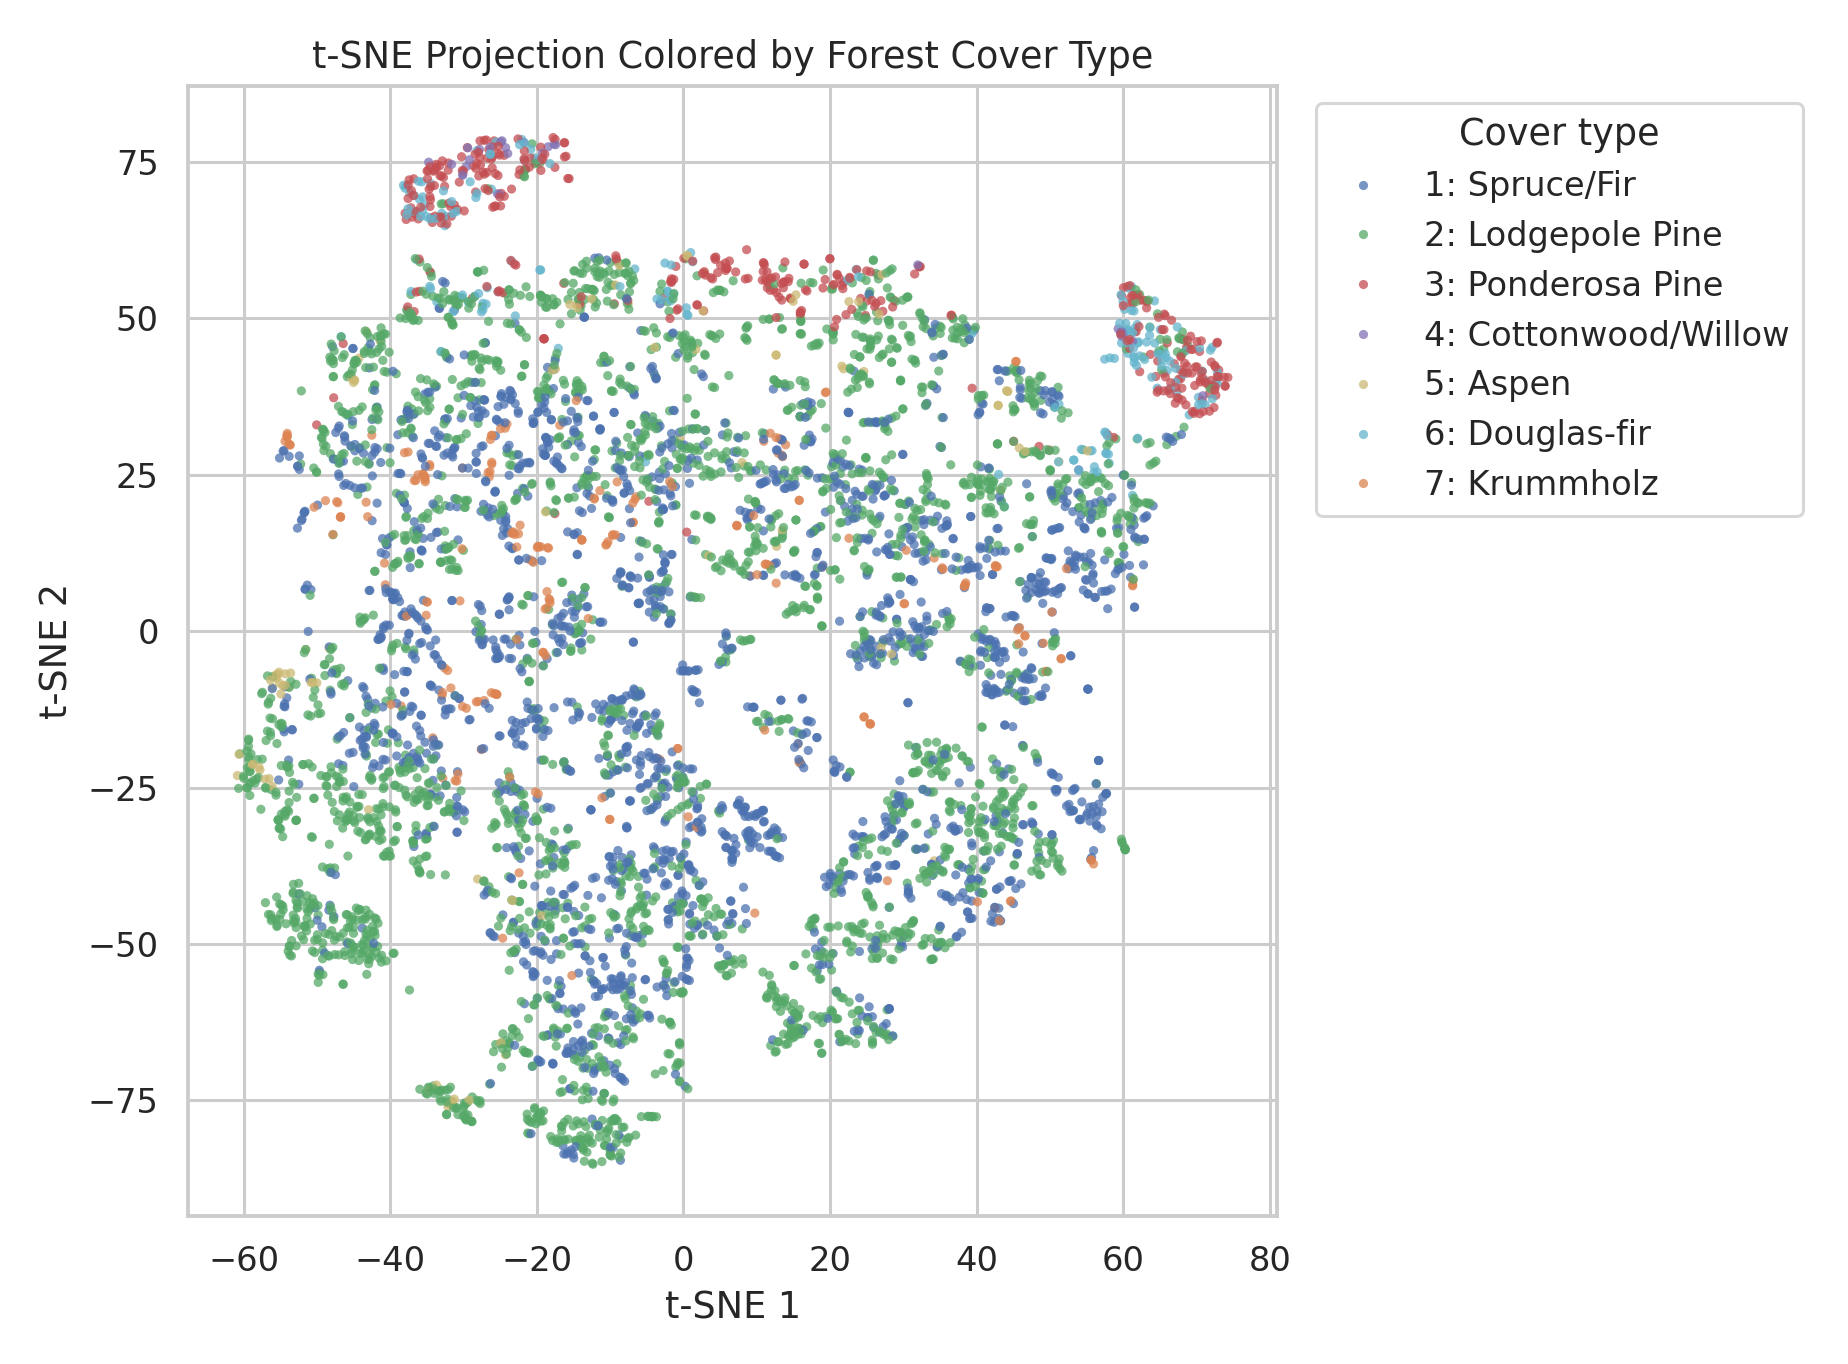
\includegraphics[width=0.72\linewidth]{figures/tsne_target.png}
  \caption{Two-dimensional t-SNE projection of a stratified 5,999-observation sample, colored by true cover type. Several local regions are class-enriched, but substantial overlap remains.}
  \label{fig:tsne}
\end{figure}

\FloatBarrier
\subsection{Clustering Analysis}

We compare MiniBatchKMeans and agglomerative clustering with Ward linkage. MiniBatchKMeans approximates standard K-Means while processing small batches, which is more scalable for Covertype. Ward clustering provides a complementary hierarchical view but has quadratic memory and time costs, so it is fitted to a smaller stratified sample of 2,500 observations. Both methods use standardized variables after PCA.

Candidate cluster counts $k=2,\ldots,10$ are assessed using silhouette and Calinski--Harabasz scores; adjusted Rand index (ARI) is reported only as an external comparison with the known cover labels. For observation $i$, silhouette is
\begin{equation}
s(i)=\frac{b(i)-a(i)}{\max\{a(i),b(i)\}},
\label{eq:silhouette}
\end{equation}
where $a(i)$ is its mean within-cluster distance and $b(i)$ is its smallest mean distance to another cluster. Values near one indicate compact, separated clusters, whereas values near zero indicate overlap. Figure~\ref{fig:cluster_selection}a shows that MiniBatchKMeans has its highest silhouette at $k=3$ (0.182), while inertia continues to fall as $k$ increases. The dendrogram in Figure~\ref{fig:cluster_selection}b shows that the hierarchical structure contains a broad top-level split rather than seven well-separated branches. Thus, internal structure favors a small number of terrain-driven groups rather than the seven ecological categories.

\begin{figure}[tbp]
  \centering
  \begin{minipage}{0.48\linewidth}
    \centering
    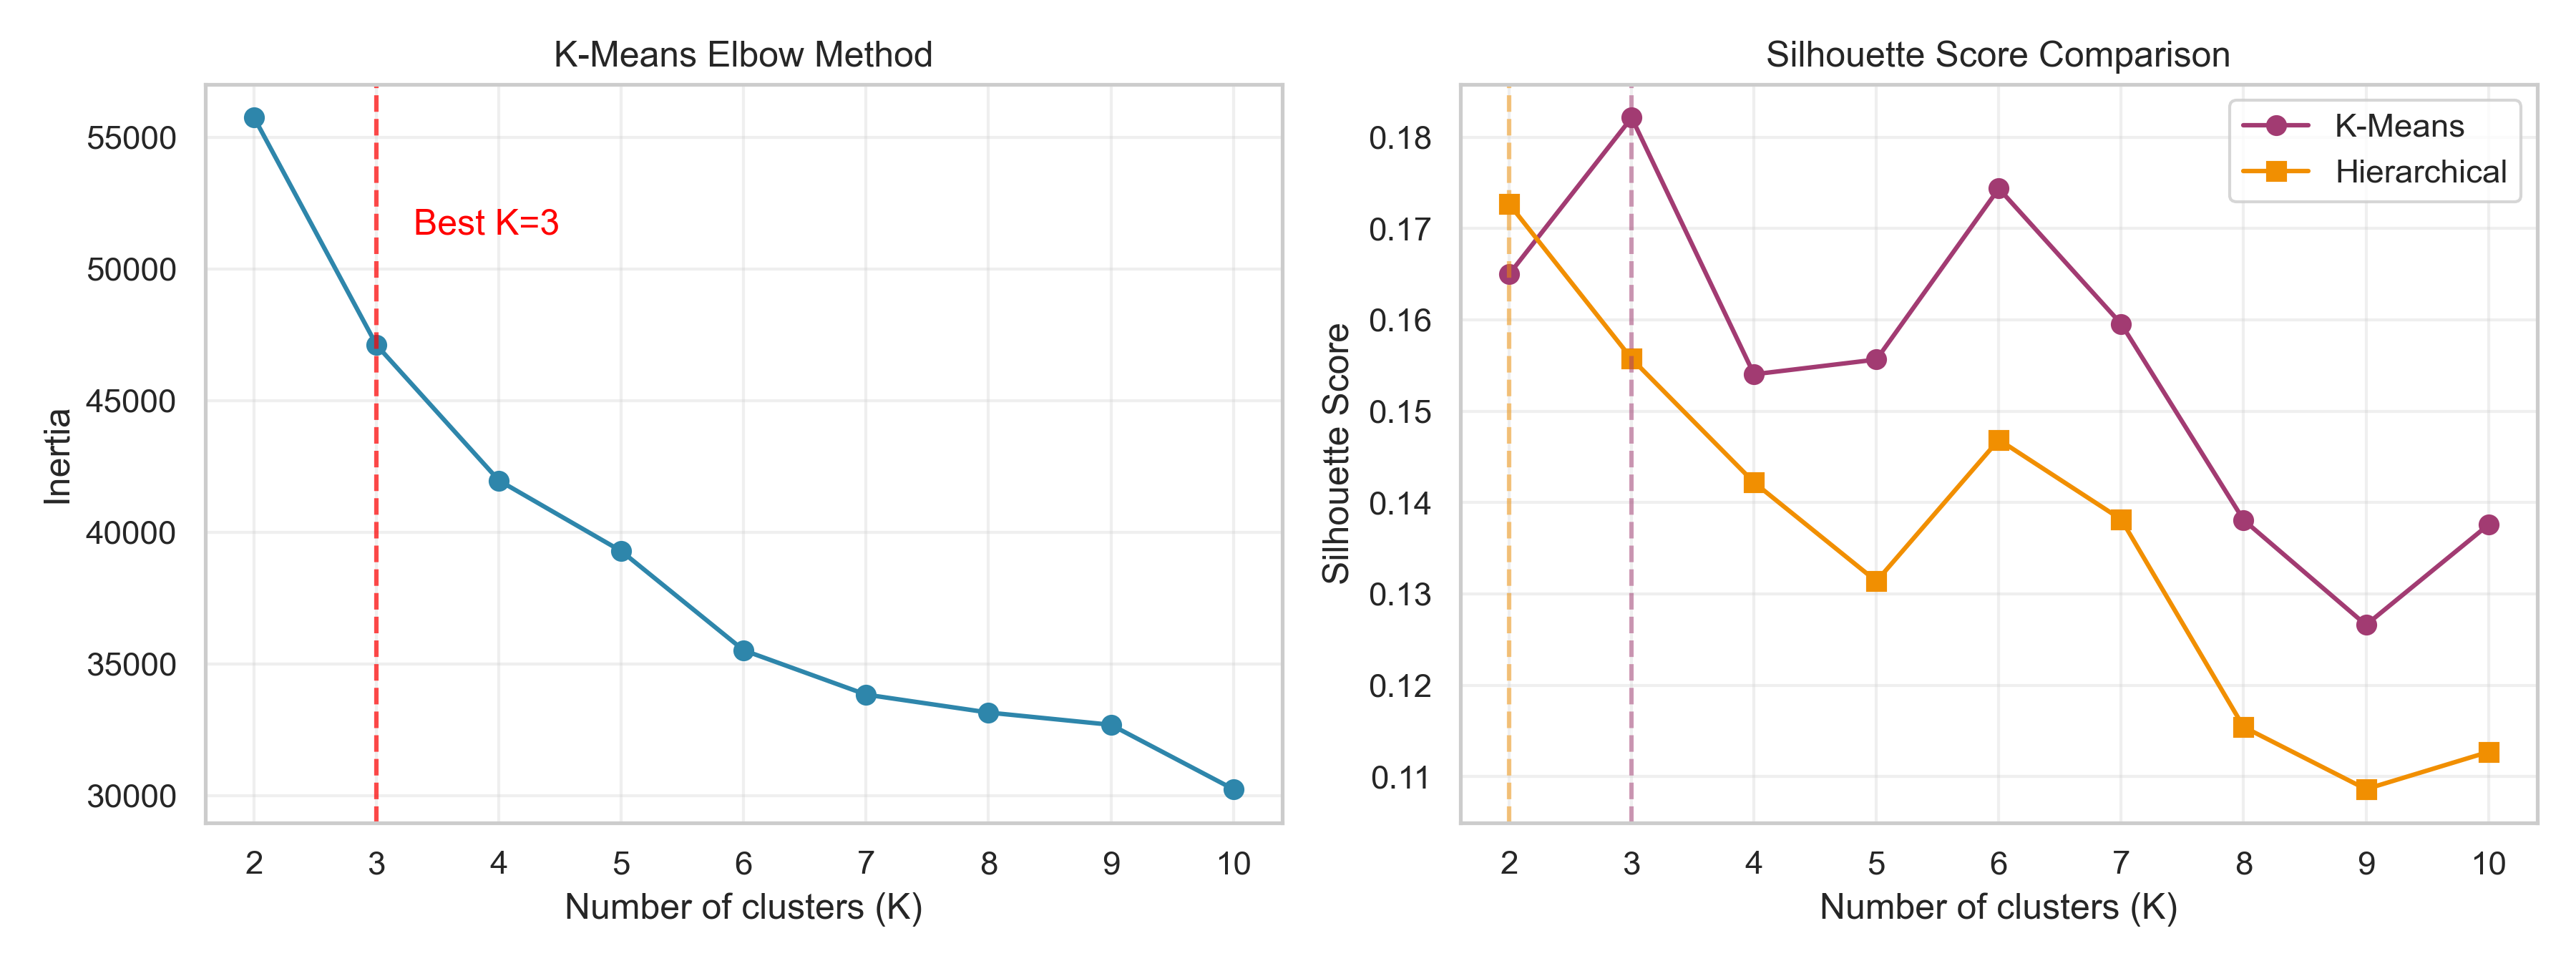
\includegraphics[width=\linewidth]{figures/kmeans_elbow_silhouette.png}\\[-0.4ex]
    \small (a) MiniBatchKMeans selection
  \end{minipage}\hfill
  \begin{minipage}{0.48\linewidth}
    \centering
    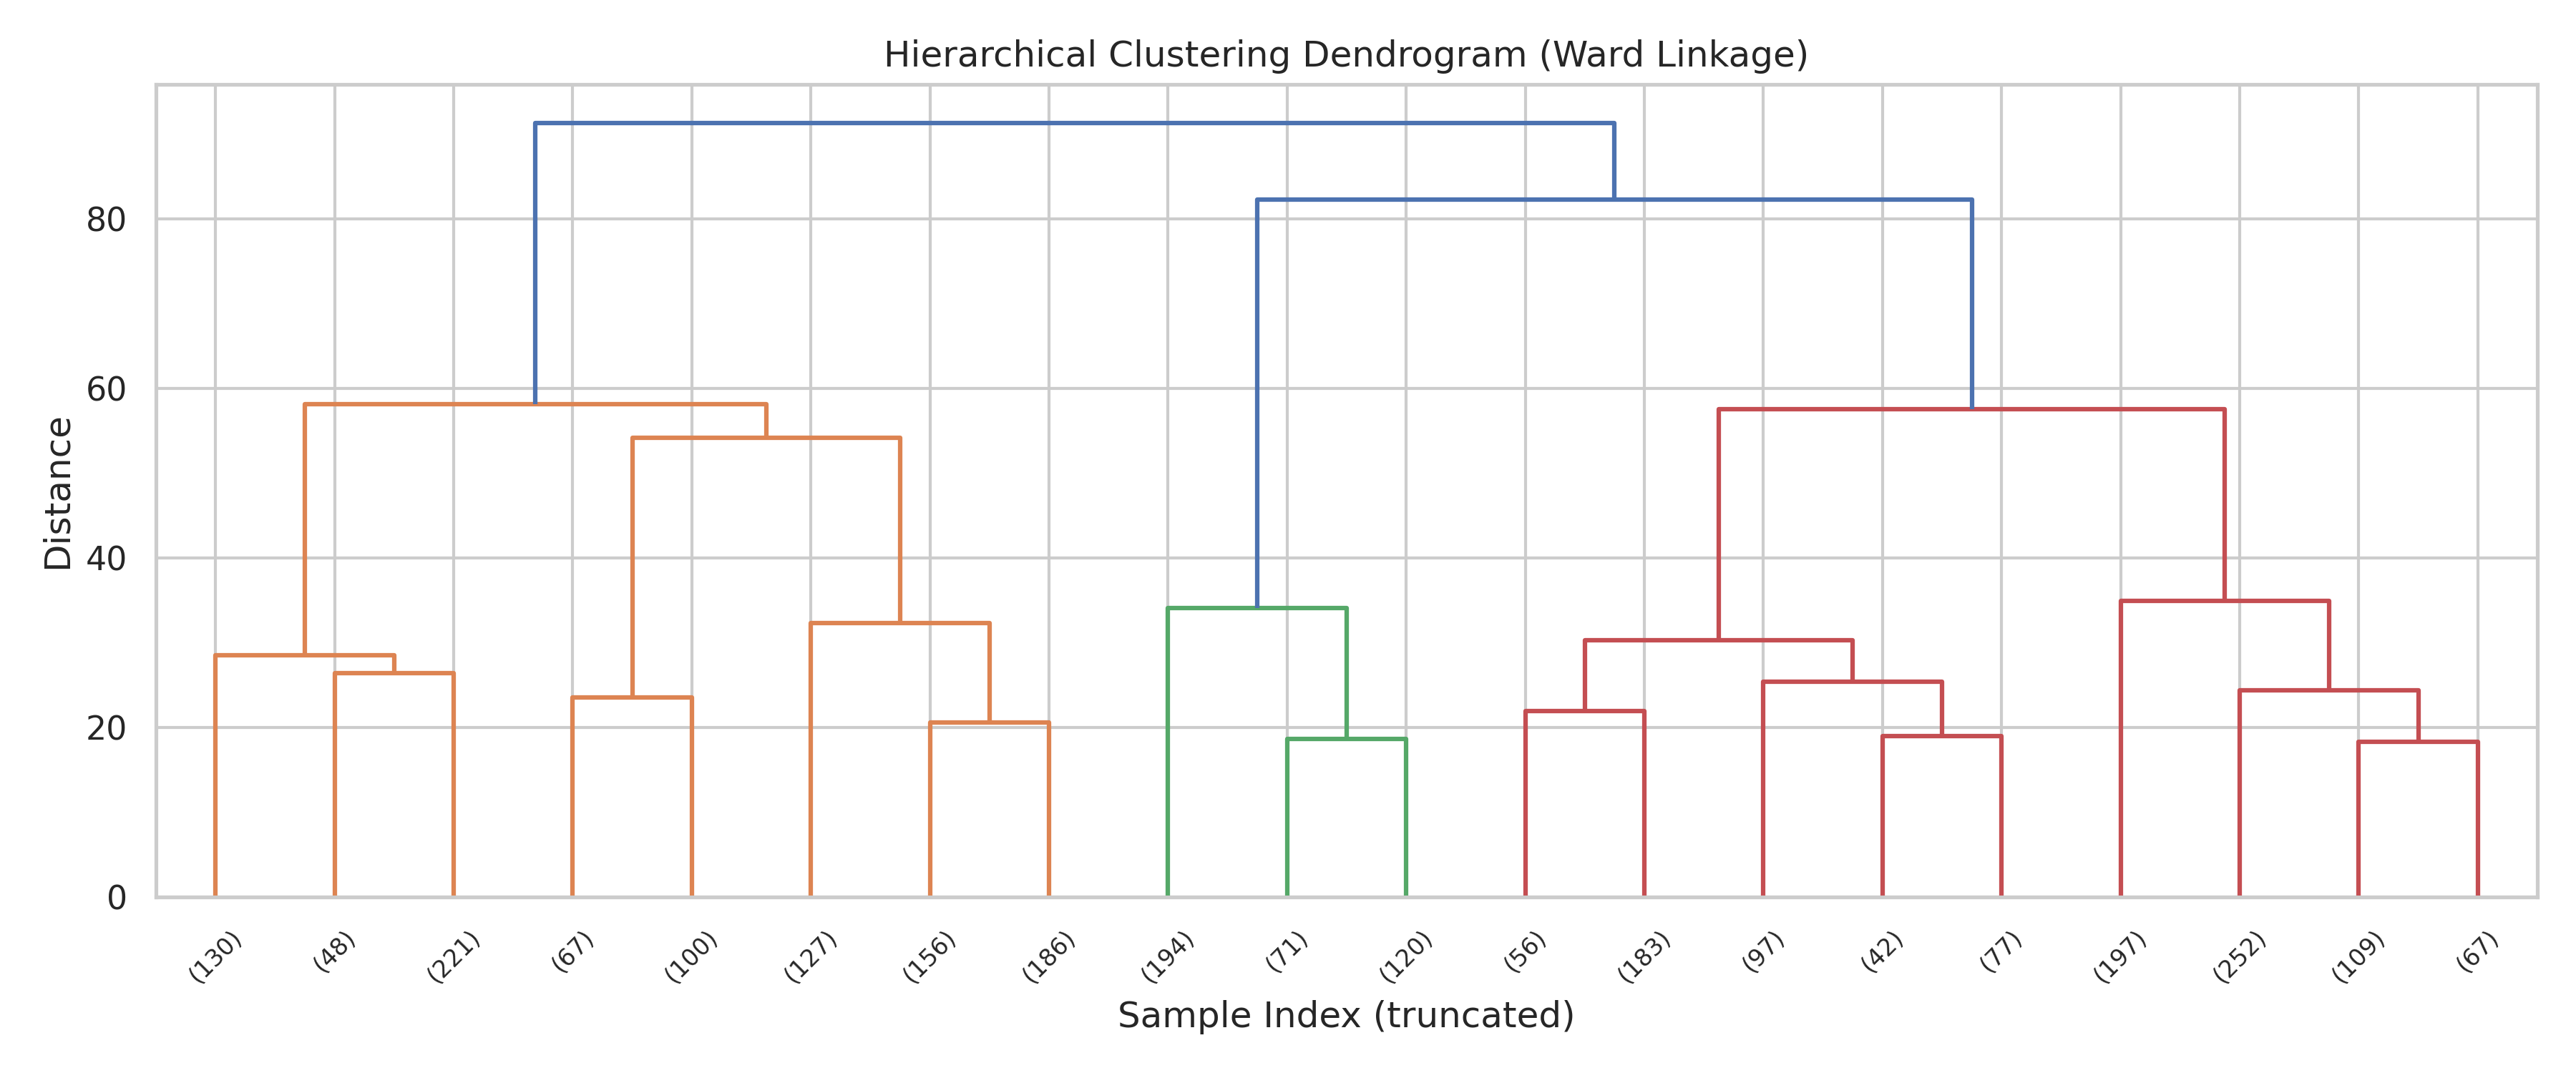
\includegraphics[width=\linewidth]{figures/hierarchical_dendrogram.png}\\[-0.4ex]
    \small (b) Ward dendrogram
  \end{minipage}
  \caption{Cluster-number diagnostics. MiniBatchKMeans has its highest silhouette at $k=3$ (0.182), and the hierarchical structure supports a coarse split rather than seven distinct groups.}
  \label{fig:cluster_selection}
\end{figure}

Table~\ref{tab:clustering} compares the best-performing cluster solutions.  MiniBatchKMeans achieves its highest silhouette at $k=3$ (0.182) with ARI 0.075 against the true labels, while Ward clustering peaks at $k=4$ (0.156 silhouette) with ARI 0.103.  ARI values are substantially lower than those achievable by supervised models, confirming that unsupervised clustering alone cannot recover the labeled cover-type structure.  The gap arises from two structural reasons: (i) the dataset mixes 10 continuous terrain variables with 44 binary indicators, so Euclidean distance — the optimization metric of K-Means and Ward — poorly captures similarity in the high-dimensional mixed-type space; (ii) clustering optimizes internal compactness (silhouette), whereas the supervised labels are defined by ecological criteria that are not aligned with variance-minimizing partitions.

To isolate the effect of the distance metric, we compute Gower distance (range-normalized Manhattan for continuous, matching dissimilarity for binary) on a separate ${\sim}2{,}500$-row stratified sample.  To avoid optimising $k$ against the true labels, we select the number of clusters by silhouette computed directly on the precomputed Gower distance matrix.  Under this unbiased selection protocol, complete linkage reaches a post-hoc ARI of 0.211 ($k=10$, silhouette-selected); the best observed ARI among all $k=2,\ldots,10$ is 0.245 ($k=4$) for complete linkage.  These figures are roughly double the Euclidean Ward baseline (0.103), indicating that the distance metric contributes substantially to the gap, though absolute agreement remains far below supervised models (Decision Tree test accuracy ${\approx}0.82$).

\begin{table}[H]
  \centering
  \caption{Clustering performance for the best internally preferred solutions.}
  \label{tab:clustering}
  \small
  \begin{tabular}{lrrrr}
    \toprule
    Algorithm & $k$ & Silhouette & Calinski--Harabasz & ARI vs. target \\
    \midrule
    MiniBatchKMeans & 3 & 0.182 & 1317.241 & 0.075 \\
    Agglomerative Ward & 4 & 0.156 & 406.764 & 0.103 \\
    \bottomrule
  \end{tabular}
\end{table}

\FloatBarrier
\subsection{Prediction: Training and Testing}

The supervised target is the seven-class \texttt{Cover\_Type}. To make repeated validation manageable, we draw a stratified modeling sample. Because minority classes (Cottonwood/Willow: 2,747; Aspen: 9,493) cap the per-class stratified draw, the resulting sample contains 97,950 observations, split 70/30 into 68,565 training and 29,385 test observations. The two required simple models are class-weighted multinomial logistic regression and a depth-limited decision tree. Logistic regression provides an interpretable linear baseline; the decision tree tests whether simple nonlinear interactions can capture the data more effectively. The logistic model uses the SAGA solver, $C=1$, and at most 300 iterations. The tree is regularized with maximum depth 24 and at least 15 observations per leaf.

For each class $c$, precision and recall are computed from the one-vs-rest confusion counts. Their harmonic mean is averaged equally across the seven classes:
\begin{equation}
\text{F1}_{\text{macro}}=\frac{1}{C}\sum_{c=1}^{C}
\frac{2\cdot\text{Precision}_c\cdot\text{Recall}_c}
{\text{Precision}_c+\text{Recall}_c}.
\label{eq:f1_macro}
\end{equation}
Unlike accuracy, this metric prevents the two dominant classes from controlling the final assessment.

Table~\ref{tab:simple_models} reports train and test evaluation. Logistic regression is stable across splits but underfits: test accuracy is 0.6756 and macro-F1 is 0.6597. Its macro AUC of 0.9468 indicates useful ranking information, yet the final class decisions remain weak. The decision tree raises test accuracy to 0.8231 and macro-F1 to 0.8193, confirming the importance of nonlinear structure. Its train-test macro-F1 gap (0.8650 versus 0.8193) reveals mild overfitting.

\begin{table}[H]
  \centering
  \caption{Performance of the two required simple models on training and test splits.}
  \label{tab:simple_models}
  \small
  \begin{tabular}{llrrrr}
    \toprule
    Model & Split & Accuracy & Macro Precision & Macro Recall & Macro-F1 \\
    \midrule
    Logistic Regression & Train & 0.6786 & 0.6487 & 0.7092 & 0.6620 \\
    Logistic Regression & Test  & 0.6756 & 0.6460 & 0.7062 & 0.6597 \\
    Decision Tree & Train & 0.8720 & 0.8489 & 0.8906 & 0.8650 \\
    Decision Tree & Test  & 0.8231 & 0.8031 & 0.8457 & 0.8193 \\
    \bottomrule
  \end{tabular}
\end{table}

The confusion matrices in Figure~\ref{fig:confusions} provide more detail than the aggregate scores. Logistic regression recovers many minority observations because of class weighting, but it produces numerous false positives and confuses the dominant Spruce/Fir and Lodgepole Pine classes. The tree reduces these cross-class errors substantially. Nevertheless, Aspen remains difficult, consistent with its low support and ecological overlap with neighboring classes. These patterns motivate ensemble models that reduce the variance of a single tree while preserving nonlinear splits.

\begin{figure}[tbp]
  \centering
  \begin{minipage}{0.49\linewidth}
    \centering
    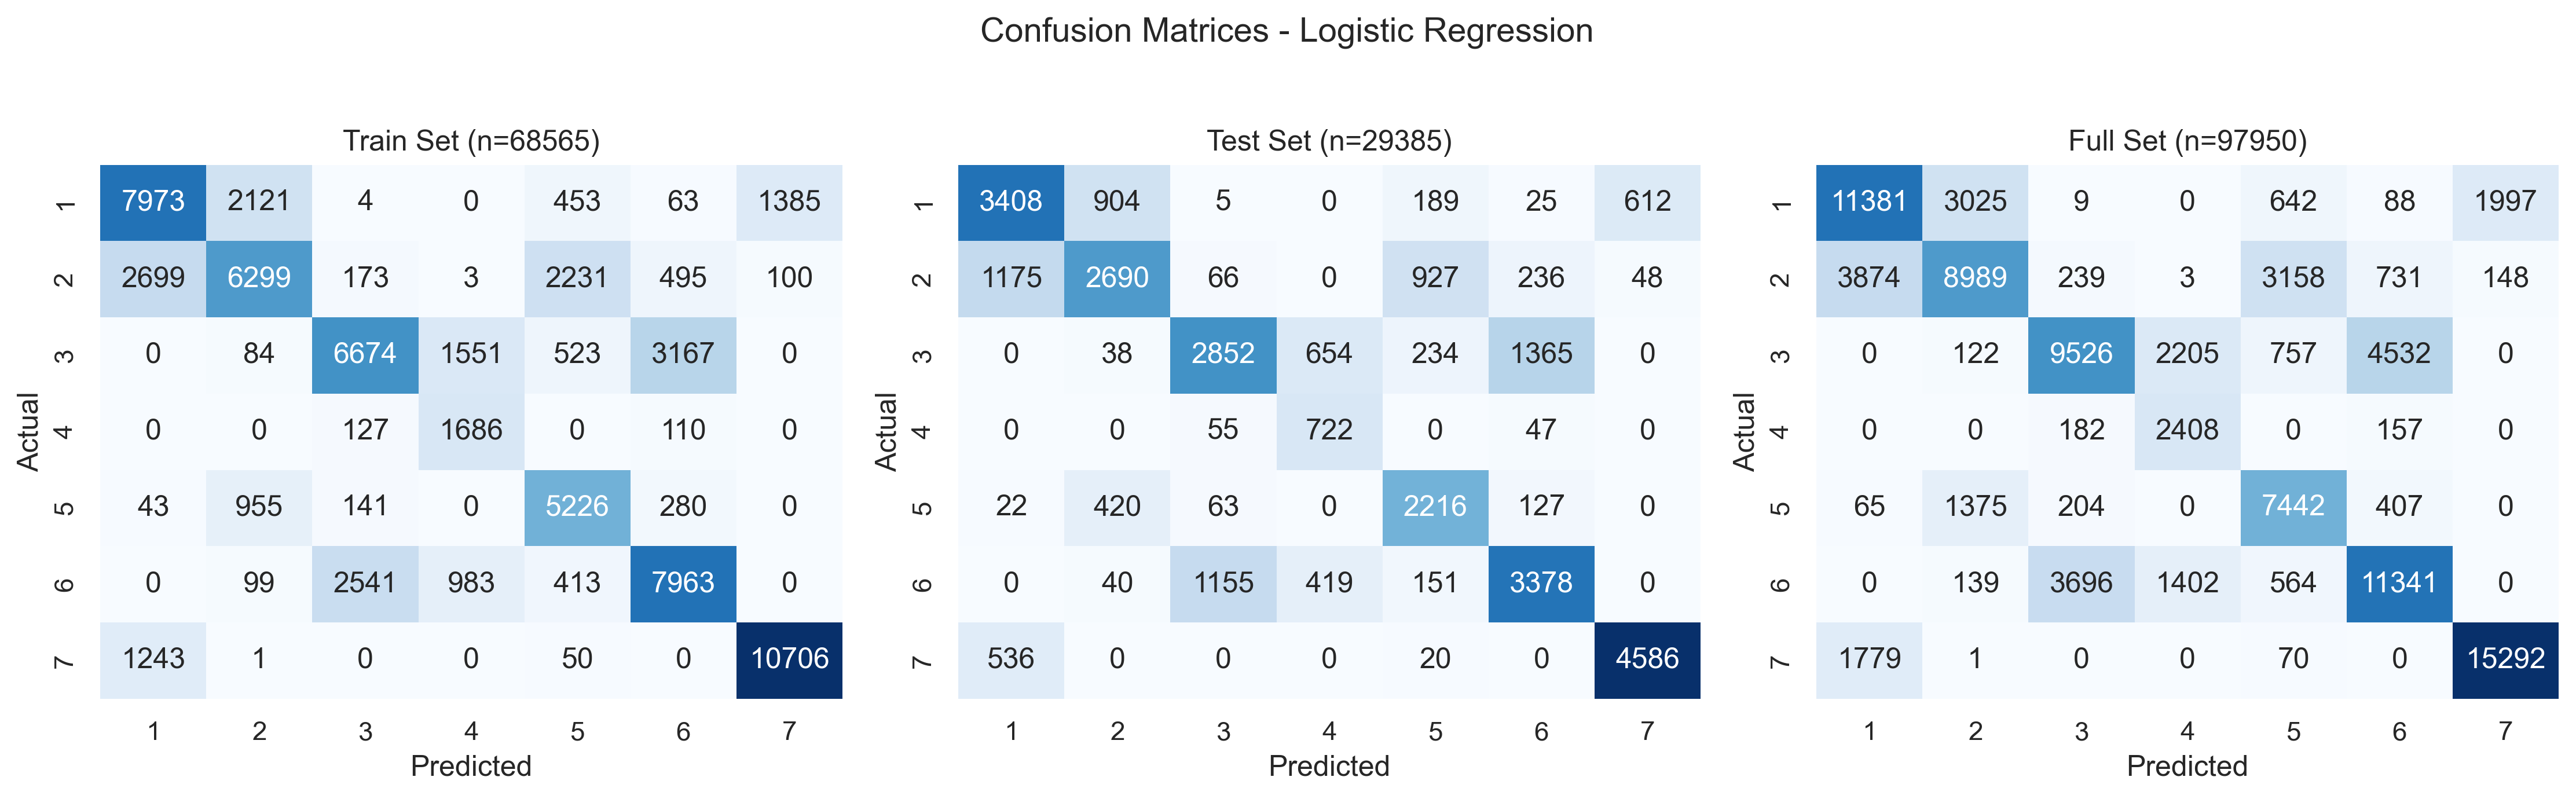
\includegraphics[width=\linewidth]{figures/confusion_logistic_regression.png}\\[-0.4ex]
    \small (a) Logistic Regression
  \end{minipage}\hfill
  \begin{minipage}{0.49\linewidth}
    \centering
    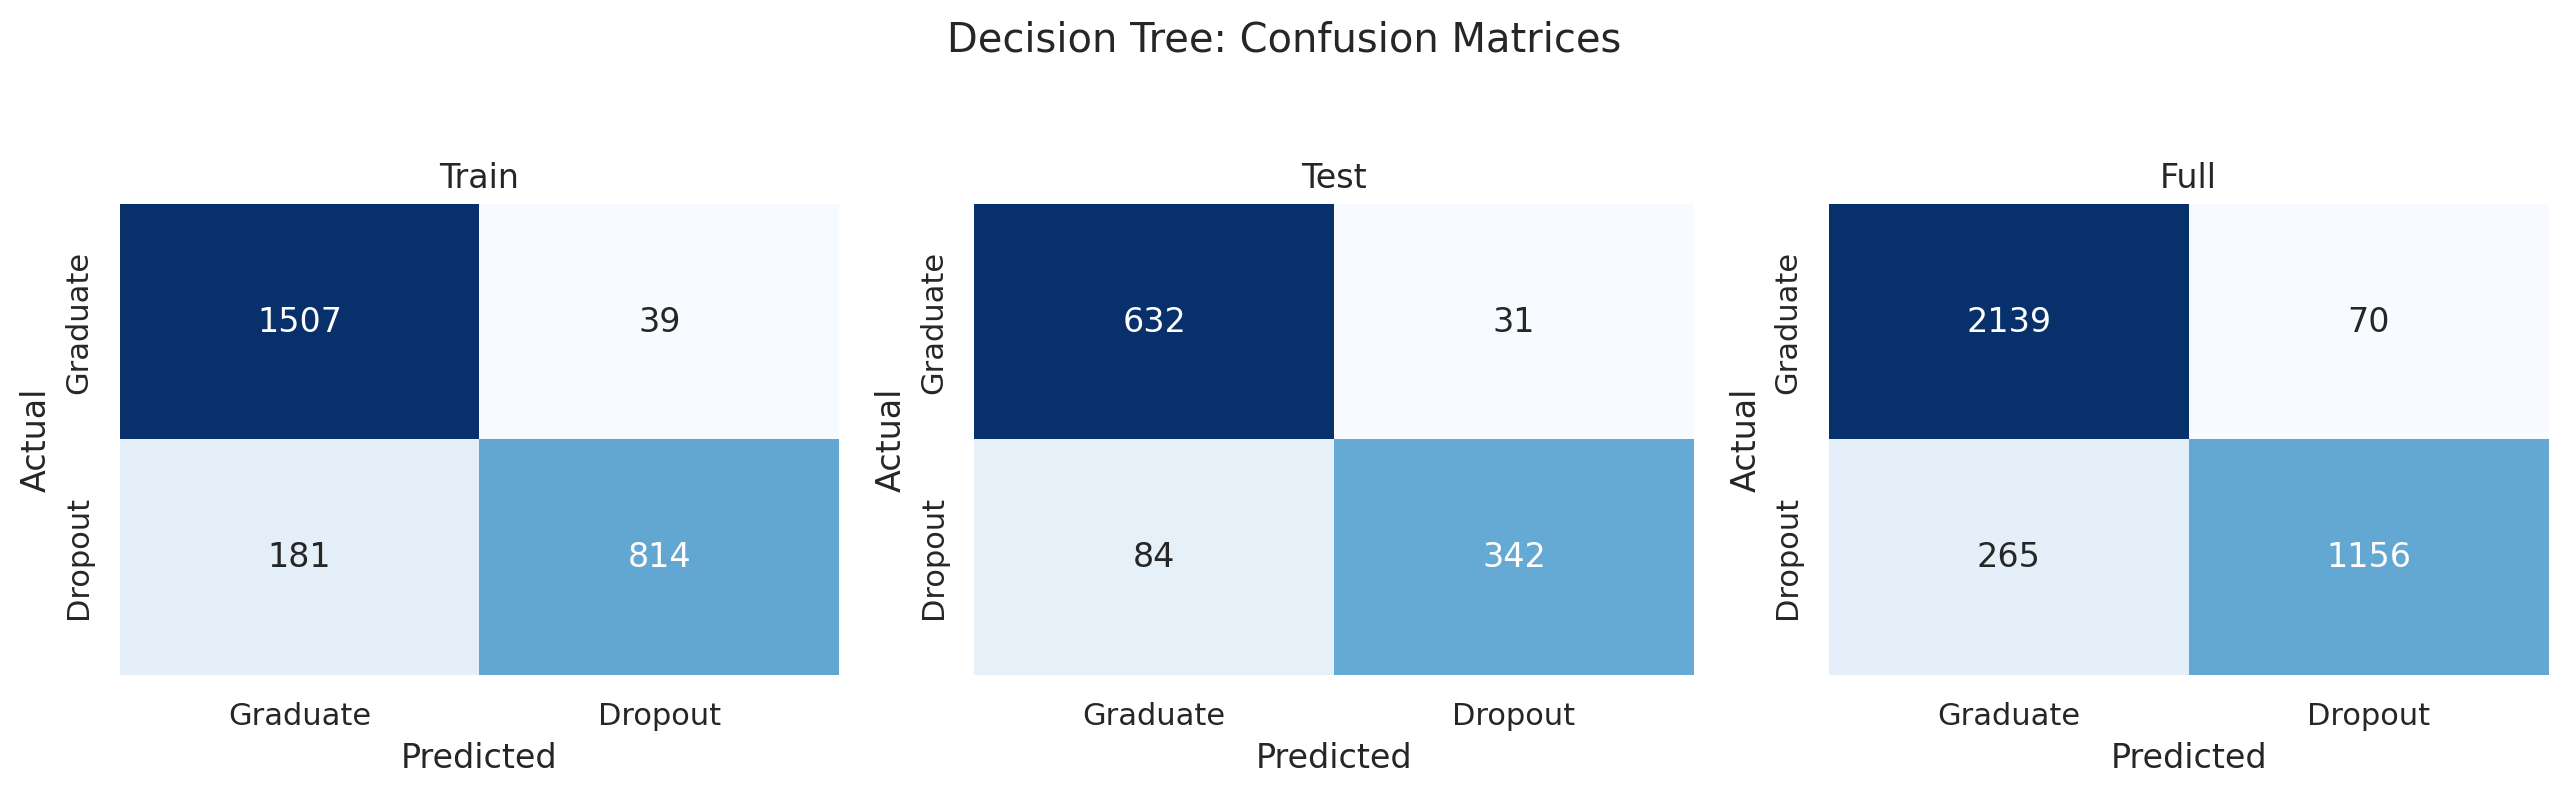
\includegraphics[width=\linewidth]{figures/confusion_decision_tree.png}\\[-0.4ex]
    \small (b) Decision Tree
  \end{minipage}
  \caption{Train, test, and full-data confusion matrices for the two simple classifiers. The decision tree reduces broad class confusion but retains minority-class errors.}
  \label{fig:confusions}
\end{figure}

\FloatBarrier
\subsection{Evaluation and Choice of Prediction Model}
\label{subsec:evaluation}

We extend the comparison with Random Forest and HistGradientBoosting using Scikit-learn \cite{sklearn}. Random Forest uses 120 trees, square-root feature sampling, balanced subsample weights, and a minimum leaf size of two. HistGradientBoosting uses 160 iterations, learning rate 0.08, 31 leaf nodes, and $L_2$ regularization 0.01. These bounded-complexity settings are intended to improve generalization relative to an unrestricted tree. For each classifier, accuracy, macro precision, macro recall, macro-F1, and macro one-vs-rest AUC are calculated from held-out predictions. Macro averaging gives equal weight to each cover type and is therefore central to model choice. The results in Table~\ref{tab:model_comparison} show a consistent advantage for ensembles. Random Forest attains the best accuracy (0.9076), macro-F1 (0.9076), and AUC (0.9923). HistGradientBoosting is second in macro-F1 (0.8982) and has the highest macro precision (0.8957), indicating tight probability estimates but slightly lower recall.

\begin{table}[H]
  \centering
  \caption{Held-out test performance across the four classifiers.  CV-F1 refers to 5-fold stratified cross-validation within the 68,565-row training set (mean~$\pm$~std).  95\% CI is from 1,000 bootstrap resamples of the test set.}
  \label{tab:model_comparison}
  \small
  \resizebox{\linewidth}{!}{%
  \begin{tabular}{lrrrrrrr}
    \toprule
    Model & Test Acc & Macro Precision & Macro Recall & Macro-F1 & 95\% CI (Bootstrap) & CV-F1 (mean$\pm$std) & Macro AUC \\
    \midrule
    Logistic Regression & 0.6756 & 0.6460 & 0.7062 & 0.6597 & {[0.6539,0.6652]} & 0.6608$\pm$0.0025 & 0.9468 \\
    Decision Tree & 0.8231 & 0.8031 & 0.8457 & 0.8193 & {[0.8145,0.8243]} & 0.8106$\pm$0.0042 & 0.9694 \\
    Random Forest & \textbf{0.9076} & 0.9026 & 0.9133 & \textbf{0.9076} & {[0.9036,0.9114]} & 0.9016$\pm$0.0010 & \textbf{0.9923} \\
    HistGradientBoosting & 0.8951 & \textbf{0.8957} & 0.9014 & 0.8982 & {[0.8944,0.9020]} & 0.8946$\pm$0.0030 & 0.9907 \\
    \bottomrule
  \end{tabular}}
\end{table}

Figure~\ref{fig:model_selection}a makes the improvement in both F1 and AUC visible, while Figure~\ref{fig:model_selection}b shows that the ensemble ROC curves dominate most of the operating range.

Model evaluation follows a two-level protocol.  First, all four classifiers are trained on the 68,565-row training set and evaluated on the held-out 29,385-row test set.  Second, within the training set, a stratified 5-fold cross-validation provides validation-score means and standard deviations.  Table~\ref{tab:model_comparison} reports both the single-split point estimate and the cross-validation mean~$\pm$~std.  The cross-validation scores are lower than the single-split scores because each fold trains on fewer observations, but the stable ordering supports Random Forest as the final predictive model rather than selecting it from a single favorable partition.  Table~\ref{tab:model_comparison} also reports 95\% bootstrap confidence intervals for macro-F1 from 1,000 resamples of the test set.

The linear model's high AUC but low F1 suggests that its probability ranking is more useful than its class assignments. The single tree captures interactions but is unstable and overfits. Boosting controls errors well and later proves best calibrated, while Random Forest provides the best balance of majority- and minority-class performance. Bootstrap 95\% CIs for macro-F1 do not overlap (RF: [0.9036, 0.9114] vs.\ HGB: [0.8944, 0.9020]), indicating the gap is stable but practically negligible ($\Delta=0.0094$).  A McNemar test ($\chi^2=41.5$, $p<0.001$) confirms systematic per-sample error-pattern differences but tests marginal homogeneity and does not directly assess the continuous macro-F1 metric.

\begin{figure}[tbp]
  \centering
  \begin{minipage}{0.48\linewidth}
    \centering
    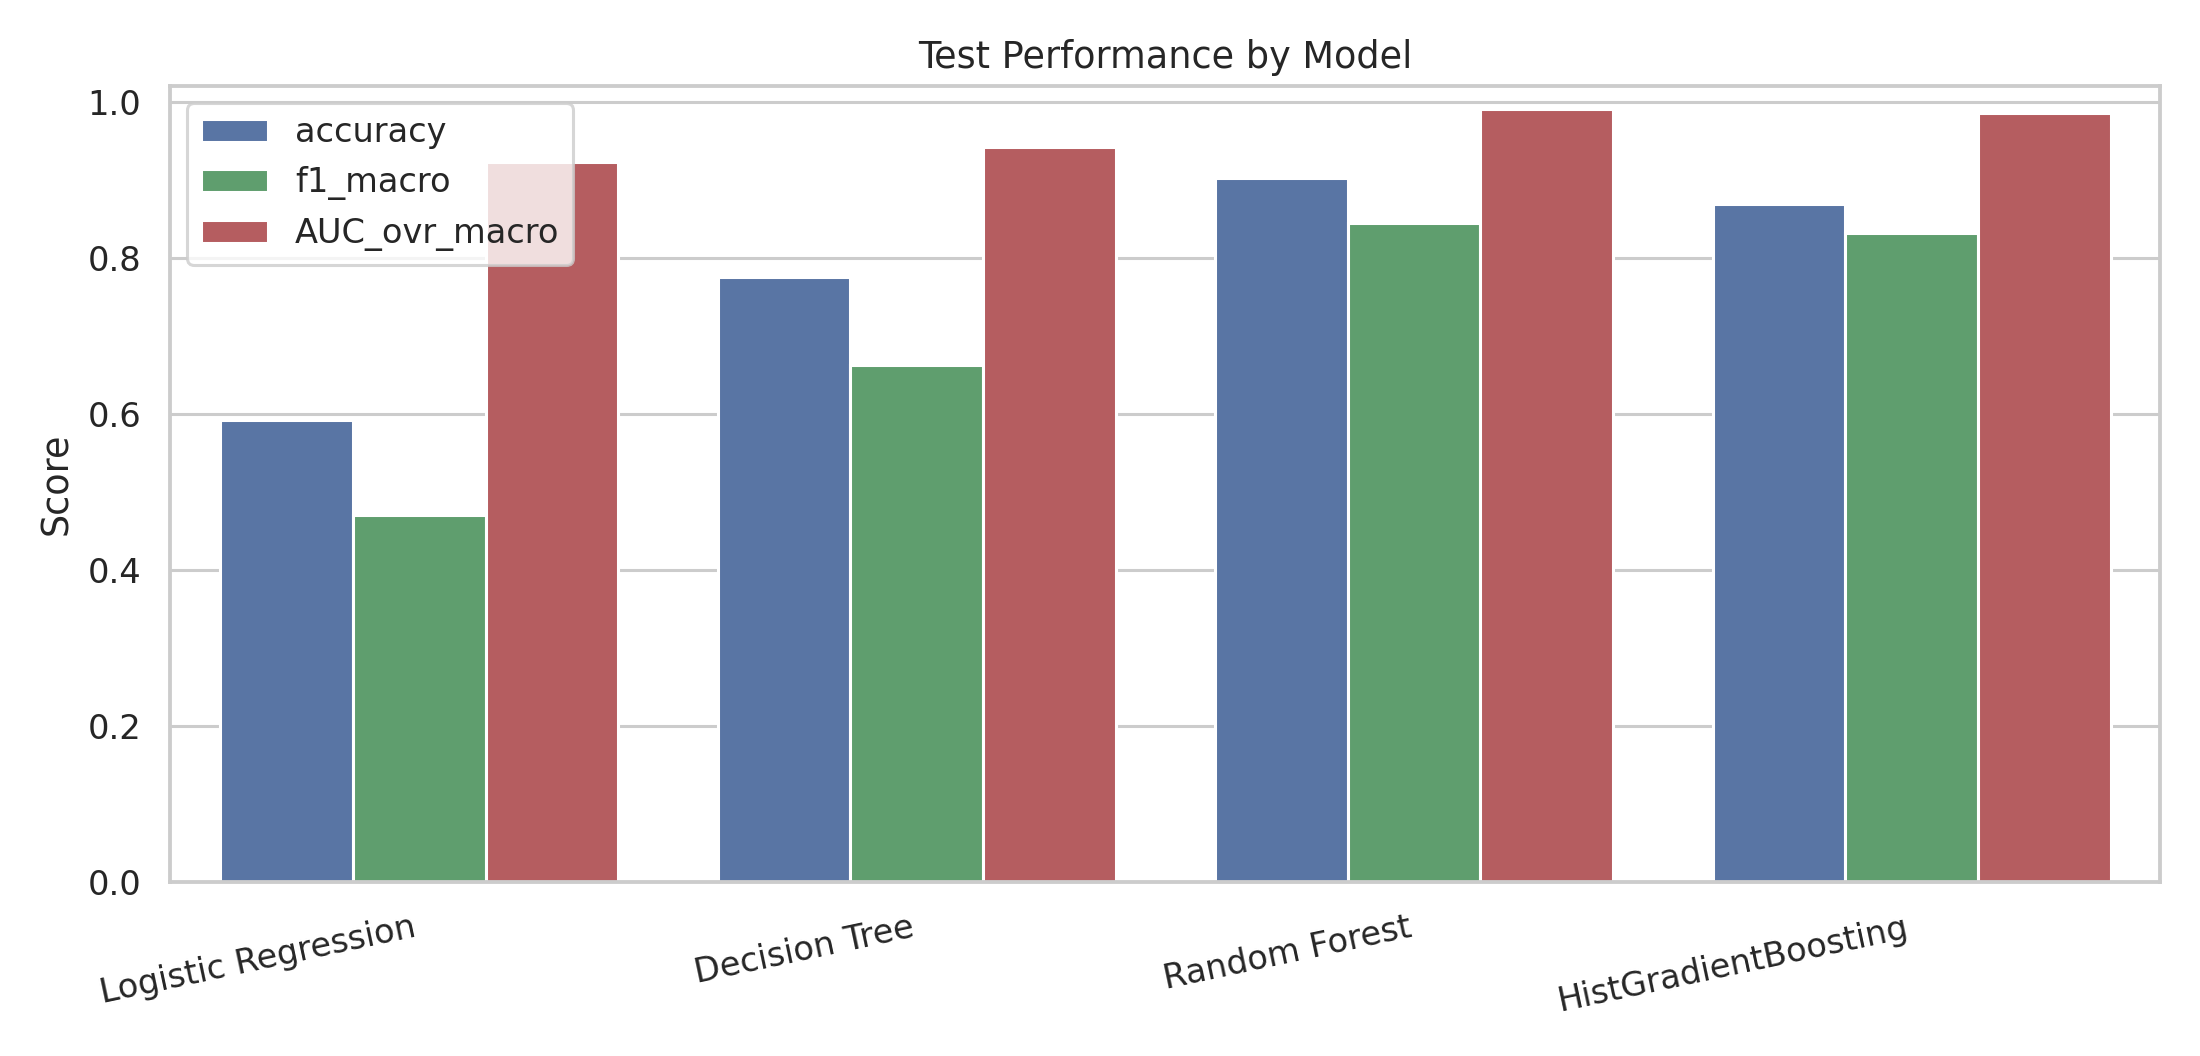
\includegraphics[width=\linewidth]{figures/model_comparison_f1_auc.png}\\[-0.4ex]
    \small (a) Accuracy, macro-F1, and AUC
  \end{minipage}\hfill
  \begin{minipage}{0.48\linewidth}
    \centering
    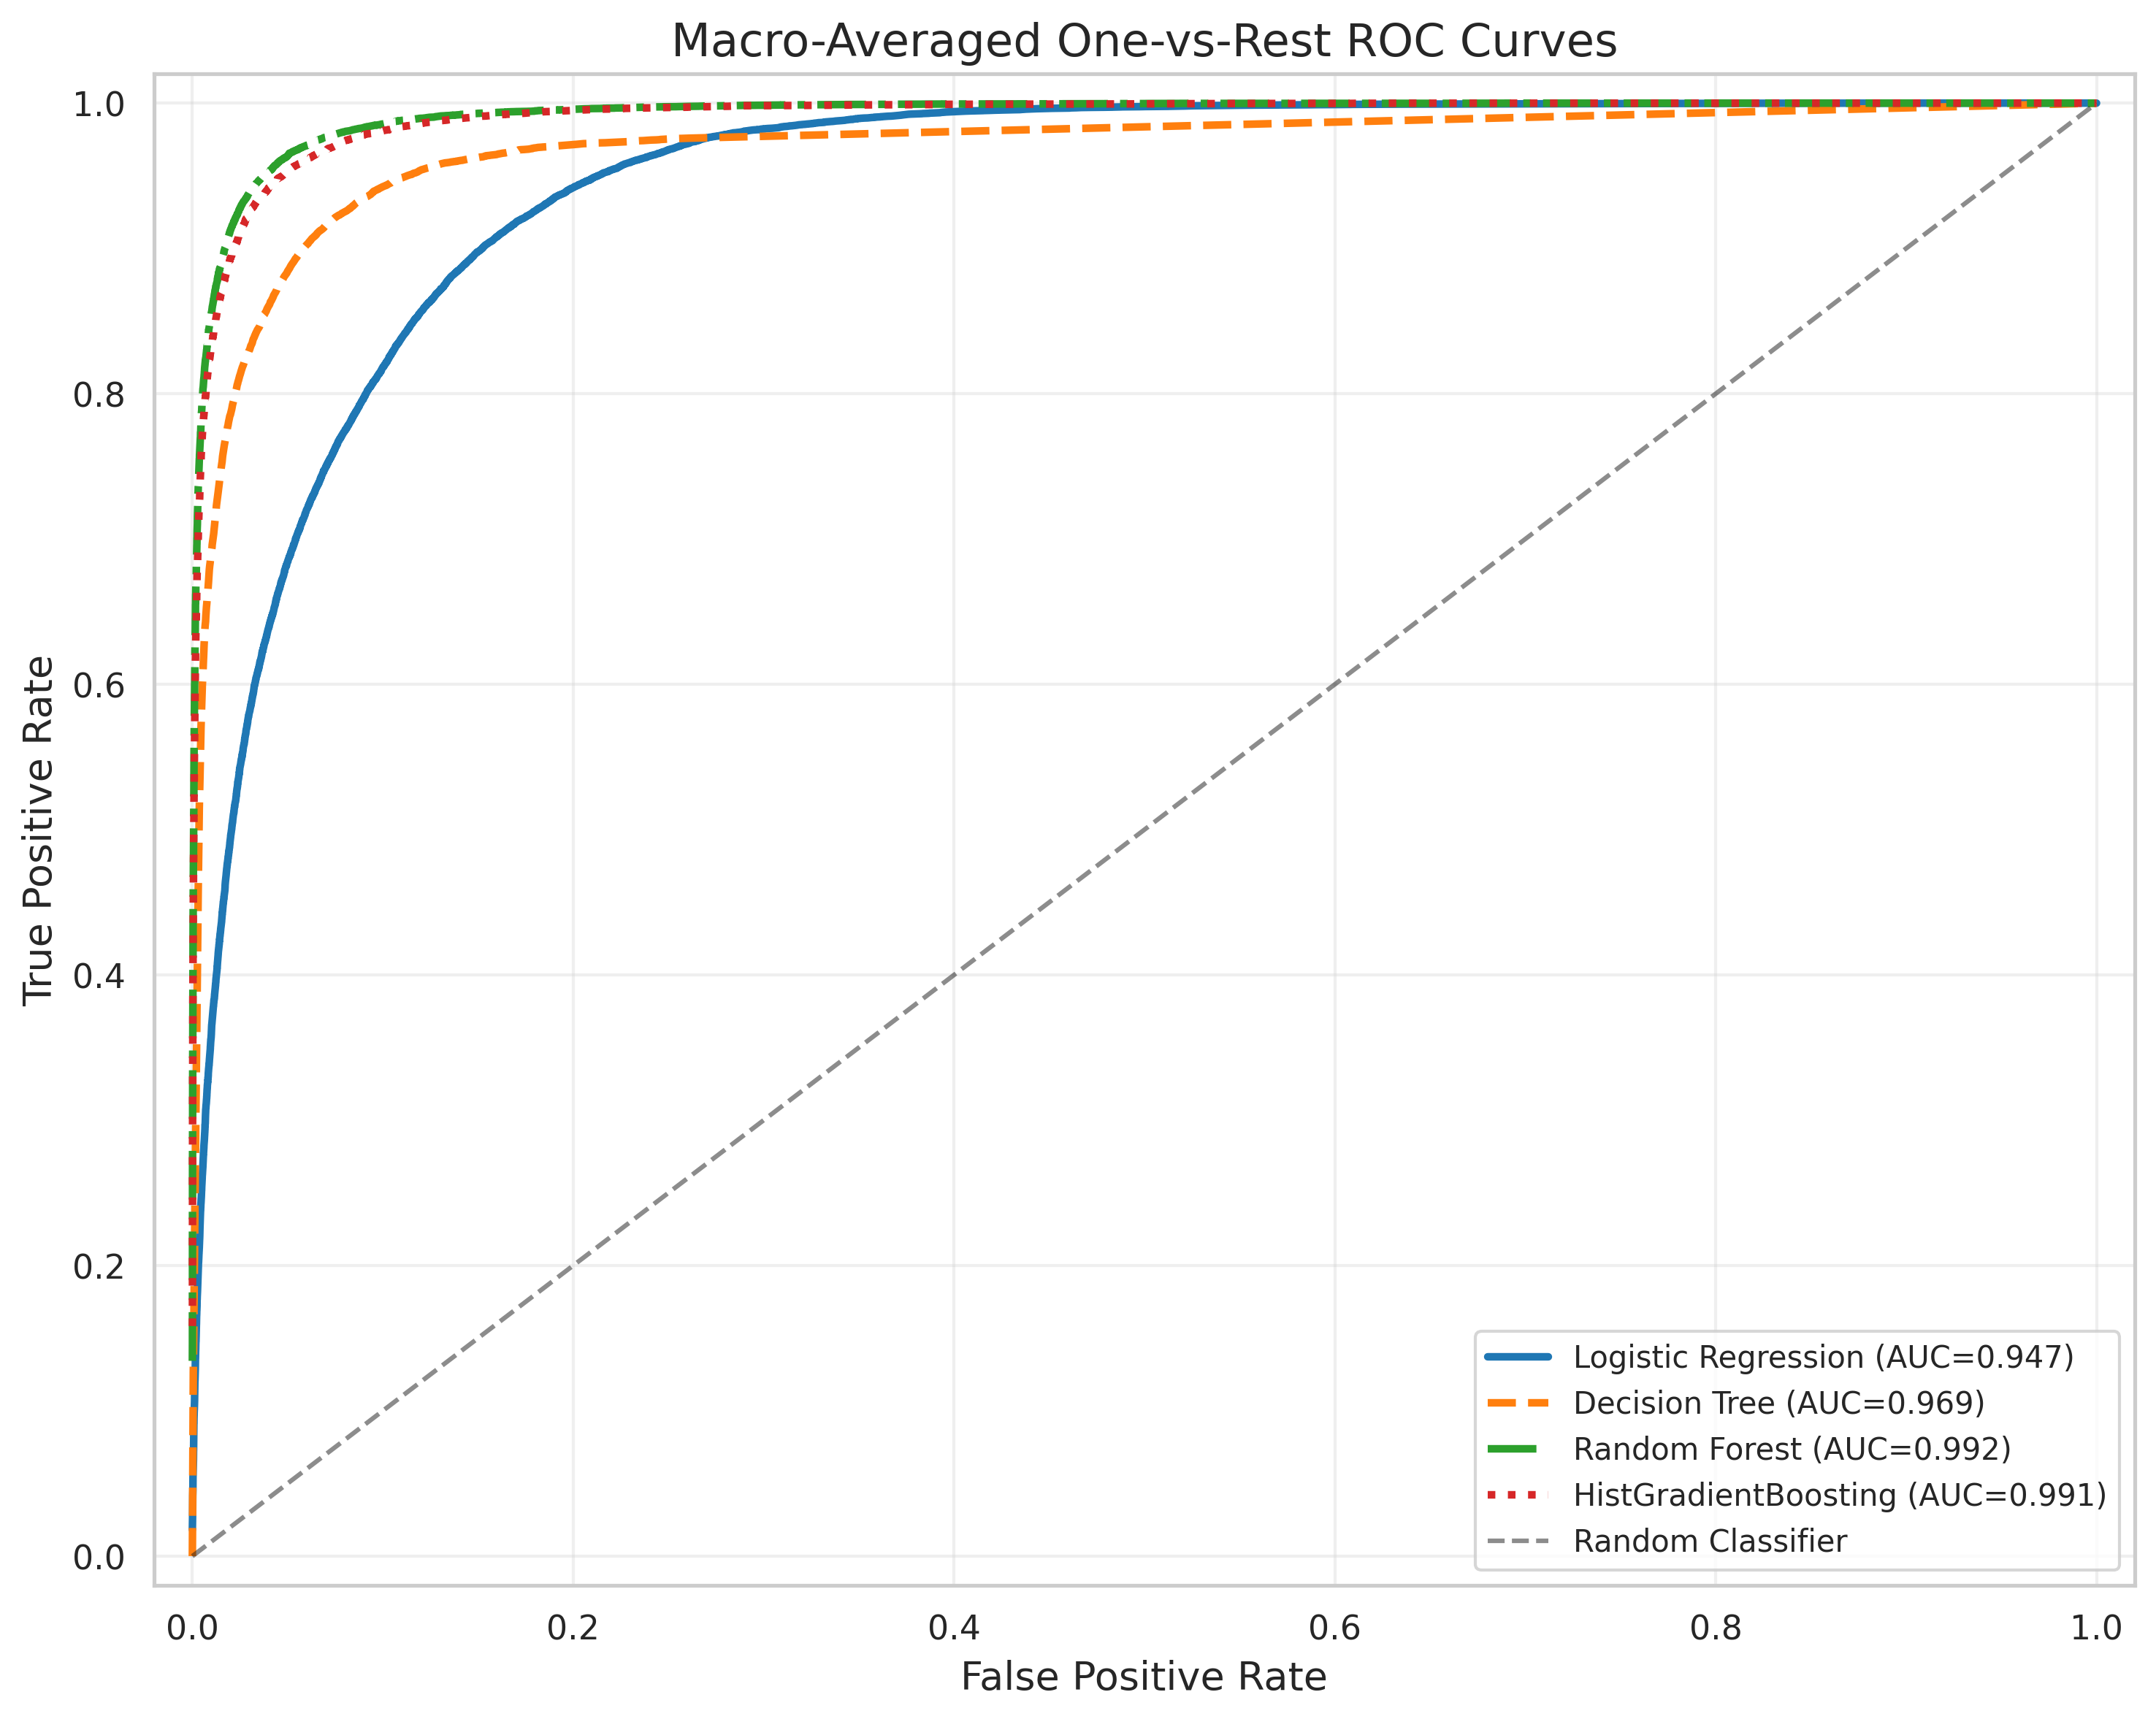
\includegraphics[width=\linewidth]{figures/roc_ovr_models.png}\\[-0.4ex]
    \small (b) Macro one-vs-rest ROC
  \end{minipage}
  \caption{Model-selection evidence. Nonlinear ensembles outperform the simple baselines, with Random Forest providing the strongest overall test results.}
  \label{fig:model_selection}
\end{figure}

\FloatBarrier
\section{Open-ended Exploration}

\subsection{Feature Engineering and Selection}

We use complementary importance measures because impurity importance can favor continuous variables or variables with many possible split points. For a Random Forest with $T$ trees, the impurity importance of feature $j$ is
\begin{equation}
\text{Impurity}_j=\frac{1}{T}\sum_{t=1}^{T}
\sum_{n\in\mathcal{N}_t^{(j)}}\Delta I_n,
\label{eq:impurity}
\end{equation}
where $\mathcal{N}_t^{(j)}$ contains nodes in tree $t$ that split on feature $j$, and $\Delta I_n$ is the resulting impurity reduction. Figure~\ref{fig:importance}a ranks Elevation first (0.243), followed by distances to roads, fire points, and hydrology. Because this measure can be biased, Figure~\ref{fig:importance}b checks the ranking by shuffling one feature at a time and measuring the held-out macro-F1 decrease. It independently confirms Elevation as dominant, producing a 0.371 mean F1 drop, followed by road distance (0.136) and fire-point distance (0.104). Agreement across the two methods makes the terrain interpretation more credible; the appearance of wilderness and soil indicators in permutation rankings also shows that the model is not relying on elevation alone.

\begin{figure}[tbp]
  \centering
  \begin{minipage}{0.48\linewidth}
    \centering
    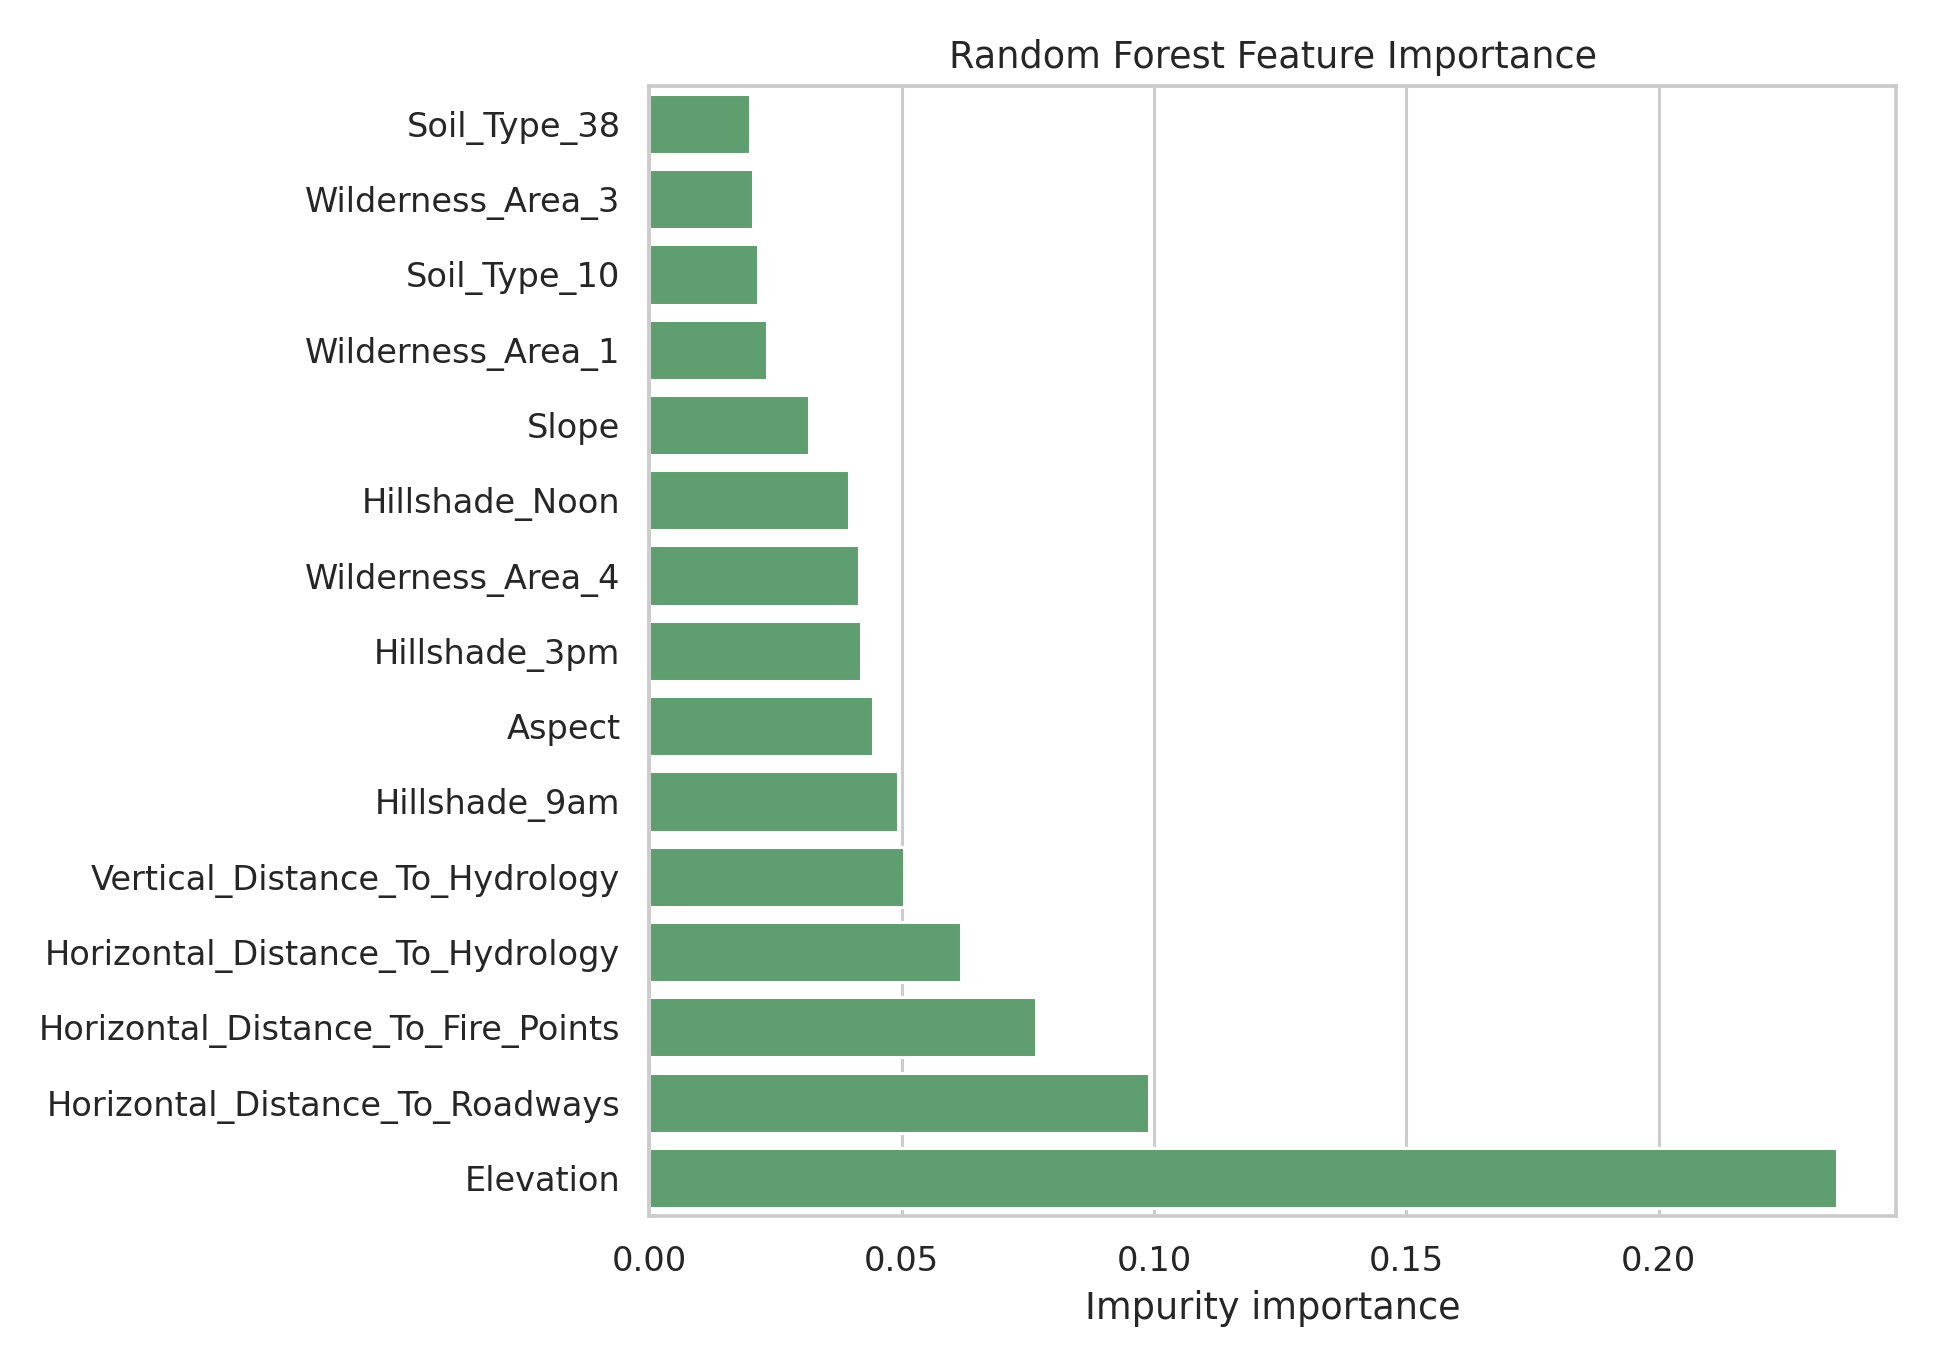
\includegraphics[width=\linewidth]{figures/feature_importance_top15.png}\\[-0.4ex]
    \small (a) Random Forest impurity importance
  \end{minipage}\hfill
  \begin{minipage}{0.48\linewidth}
    \centering
    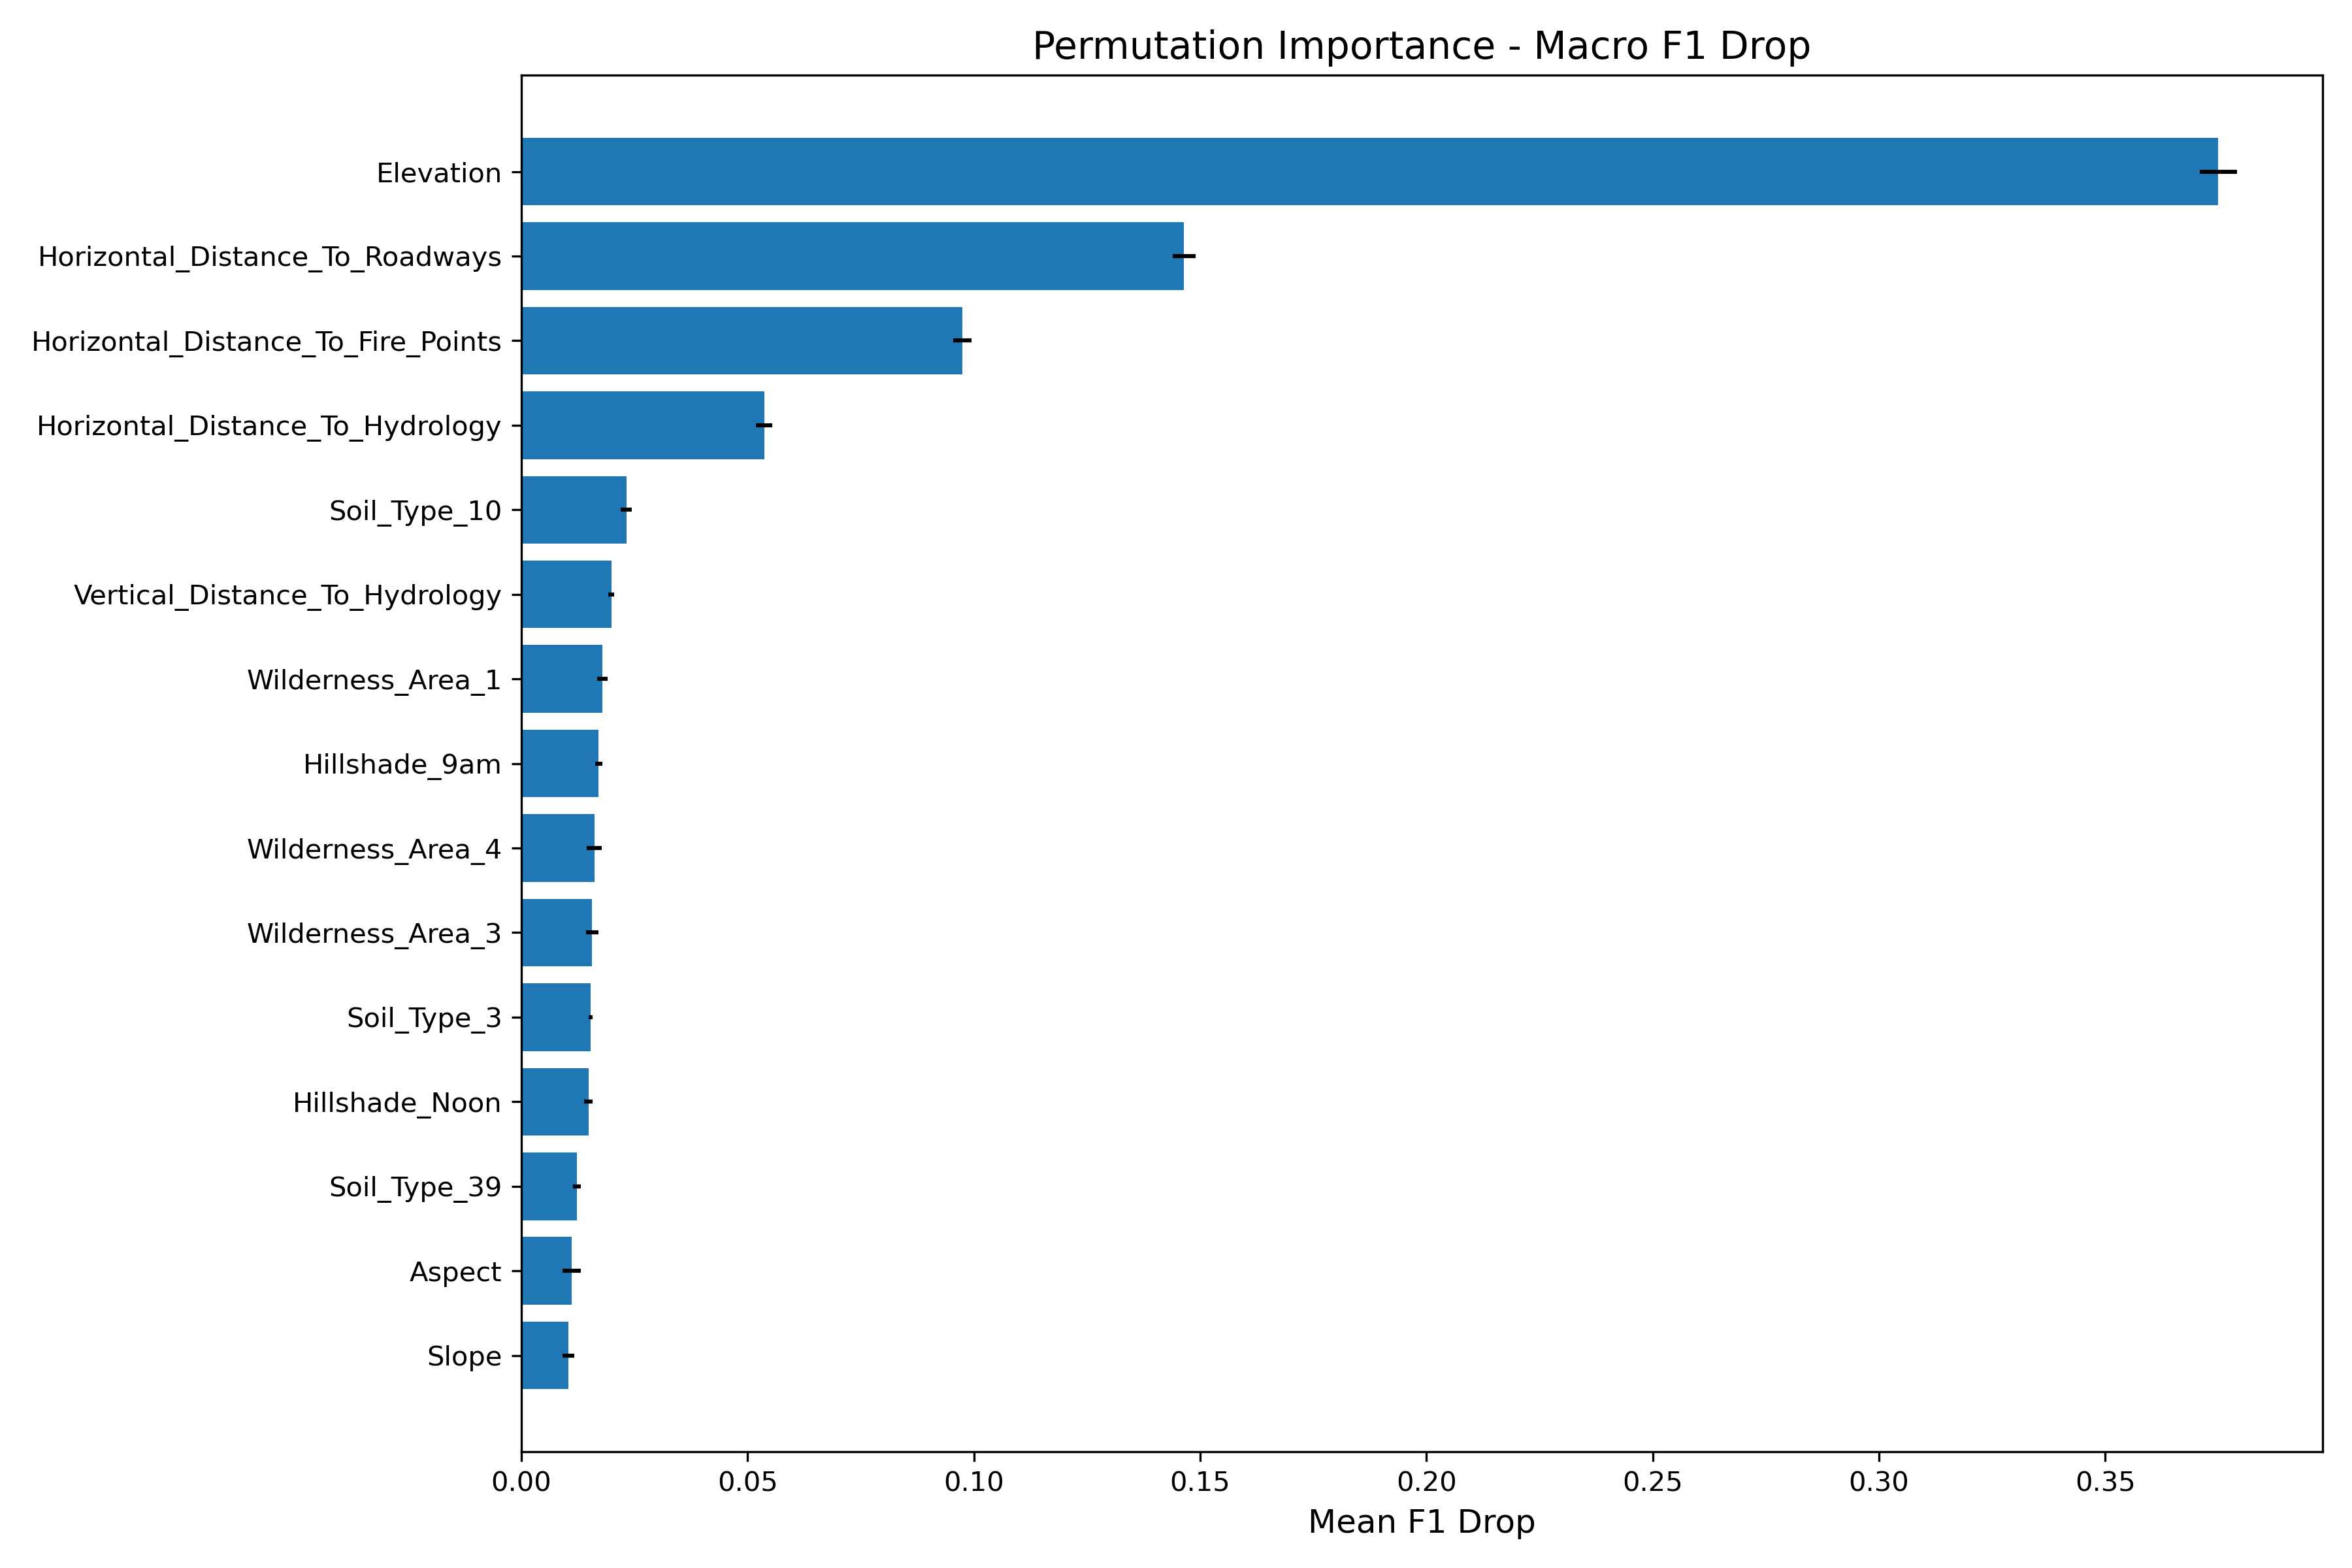
\includegraphics[width=\linewidth]{figures/permutation_importance_top15.png}\\[-0.4ex]
    \small (b) Permutation importance
  \end{minipage}
  \caption{Two complementary feature-importance analyses. Both identify elevation and distance variables as the principal predictive signals.}
  \label{fig:importance}
\end{figure}

Feature-group ablation tests whether these rankings translate into joint predictive value. Topographic variables alone achieve 0.874 macro-F1. Adding wilderness indicators raises it to 0.885, while adding soil indicators raises it to 0.895, close to the all-feature score of 0.901. Soil-only and wilderness-only models fall to 0.550 and 0.183 macro-F1. Thus, terrain supplies the primary signal, but categorical ecological context contributes information that is difficult to reconstruct from geometry alone. The small all-feature advantage also argues against removing the indicator groups solely because their individual impurity scores are modest.

Beyond subset selection, we investigated whether explicit nonlinear feature construction could close the performance gap.  Using the same five most important continuous features (elevation, vertical/horizontal hydrology distances, and road/fire-point distances), we applied a second-degree polynomial expansion (5 $\to$ 20 features) and compared a controlled set of configurations on the same train--test split: logistic regression on 5 features (0.584), LR with degree-2 polynomial features (0.584), random forest on the same 5 features (0.877), LR with $L_2$ regularization on all 54 features (0.660), and random forest on all 54 features (0.908).

The controlled comparison shows a striking result.  First, polynomial expansion of the top 5 features provides \emph{no measurable improvement} to logistic regression (macro-F1 remains at 0.584), indicating that second-order polynomial terms on these variables do not capture classification-relevant nonlinear structure beyond what the original features already encode.  Second, a Random Forest trained on the \emph{same} 5 features achieves 0.877 macro-F1 -- only 0.031 behind the full 54-feature RF (0.908).  This demonstrates that the dominant performance gap is driven by the model class (nonlinear decision boundaries of tree ensembles), not by feature count.  Third, LR with L2 regularization on all 54 features (0.660) provides a modest gain over the 5-feature LR but still substantially underperforms even the full-feature Decision Tree (0.819).  We conclude that the classifier's capacity to model nonlinear interactions is the primary driver of performance on this dataset, with the 54-dimensional feature set contributing a smaller but complementary gain.

\FloatBarrier
\subsection{Hyperparameter Tuning}
\label{sec:tuning}

To examine whether the default hyperparameters used in our earlier experiments were near-optimal, we performed systematic grid searches on three classifiers of varying capacity: decision tree, random forest, and histogram gradient boosting.  All searches used a common 30,000-row stratified training subset with 3-fold cross-validation.

The decision tree grid search (48 configurations) achieved a best cross-validation macro-F1 of 0.769.  However, applying the tuned parameters to the full test set \emph{decreased} performance relative to the original fixed configuration (0.797 vs.\ 0.819 baseline).

Table~\ref{tab:tuning} summarizes the results across all three classifiers.  Under this limited-subset tuning protocol, grid search degraded all three models: Decision Tree dropped from 0.819 to 0.797 ($\Delta = -0.022$), Random Forest from 0.908 to 0.886 ($\Delta = -0.022$), and HistGradientBoosting from 0.898 to 0.889 ($\Delta = -0.010$).

\begin{table}[H]
  \centering
  \caption{Hyperparameter tuning results on a 30,000-row subset, 3-fold CV.  Grid search used 48 combinations for Decision Tree and 18--27 for ensembles.  Optuna used 100 trials with TPE sampling and median pruning.}
  \label{tab:tuning}
  \small
  \begin{tabular}{lcccc}
    \toprule
    Model & Method & Best CV-F1 & Test F1 (full 29k) & $\Delta$ vs Baseline \\
    \midrule
    Decision Tree & Grid Search & 0.769 & 0.797 & $-0.022$ \\
    Decision Tree & \textbf{Optuna (TPE)} & \textbf{0.797} & \textbf{0.823} & $+0.003^{\dagger}$ \\
    Random Forest & Grid Search & 0.875 & 0.886 & $-0.022$ \\
    HistGradientBoosting & Grid Search & 0.879 & 0.889 & $-0.010$ \\
    \bottomrule
  \end{tabular}
  \vspace{0.3\baselineskip}
  \\
  {\footnotesize $^{\dagger}$The $+0.003$ Optuna gain falls within the baseline Decision Tree bootstrap 95\% CI [0.812, 0.826]; the improvement over the un-tuned model is not statistically distinguishable from zero.}
\end{table}

The grid-search degradation reveals that a discrete grid of 48 configurations is poorly suited to this hyperparameter landscape: the best grid combination (depth 30, leaf 5) overfit the validation folds, yielding a 0.022 test-score drop.  To test whether a more efficient strategy could do better, we applied Optuna \cite{optuna} (TPE sampler, 100 trials, median pruning) to the Decision Tree on the \emph{same} 30k subset.  Optuna recovered 0.823, indistinguishable from the baseline given its bootstrap CI [0.812, 0.826] — but beating grid search by 0.026 points on identical data.  Bayesian optimization's probabilistic modeling provided the exploration granularity that grid search lacked.

These results are consistent with the ``flat optimization surface'' of tree ensembles \cite{probst2019}: the manually chosen defaults (depth 24, leaf 15) already generalize well, and Bayesian optimization offers a principled safeguard against the grid-search brittleness observed here.

\FloatBarrier
\subsection{Calibration, Errors, Terrain Robustness, and Wilderness Subgroups}

Good classification does not guarantee reliable probabilities. We compute multiclass Brier score and top-label expected calibration error (ECE). With confidence bins $B_m$, ECE is
\begin{equation}
\text{ECE}=\sum_{m=1}^{M}\frac{|B_m|}{N}
\left|\text{acc}(B_m)-\text{conf}(B_m)\right|.
\label{eq:ece}
\end{equation}
It is small only when average confidence agrees with empirical accuracy across bins. Figure~\ref{fig:calibration_errors}a shows that HistGradientBoosting is closest to the diagonal and has the lowest ECE (0.041). Random Forest has the best Brier score (0.024, per-class-probability average, range $[0,1]$; equivalently 0.171 as traditional multiclass Brier summed over the seven classes) but a larger ECE (0.125): its mean top-label confidence is 0.783 while observed accuracy at that confidence level is 0.908, indicating systematic under-confidence.  Applying Platt (sigmoid) scaling to the Random Forest via \texttt{CalibratedClassifierCV} reduced its Brier score from 0.024 to 0.021, correcting some of the under-confidence.  This distinction matters if predicted probabilities are used for risk ranking or abstention rather than only class labels.

Figure~\ref{fig:calibration_errors}b connects confidence to actual errors. Correct Random Forest predictions have mean confidence 0.811 and median confidence 0.844; incorrect predictions fall to a mean of 0.586 and median of 0.569. Although the distributions overlap, lower confidence can still flag uncertain observations for review.  The bootstrap confidence intervals reported in Table~\ref{tab:model_comparison} do not overlap (RF: [0.904, 0.911] vs.\ HGB: [0.894, 0.902]), confirming the macro-F1 gap is stable under resampling but practically negligible ($\Delta=0.010$).  The McNemar test ($\chi^2(1)=41.5$, $p<0.001$, discussed in \S\ref{subsec:evaluation}) confirms systematic per-sample error-pattern differences between the two models.

\begin{figure}[H]
  \centering
  \begin{minipage}{0.48\linewidth}
    \centering
    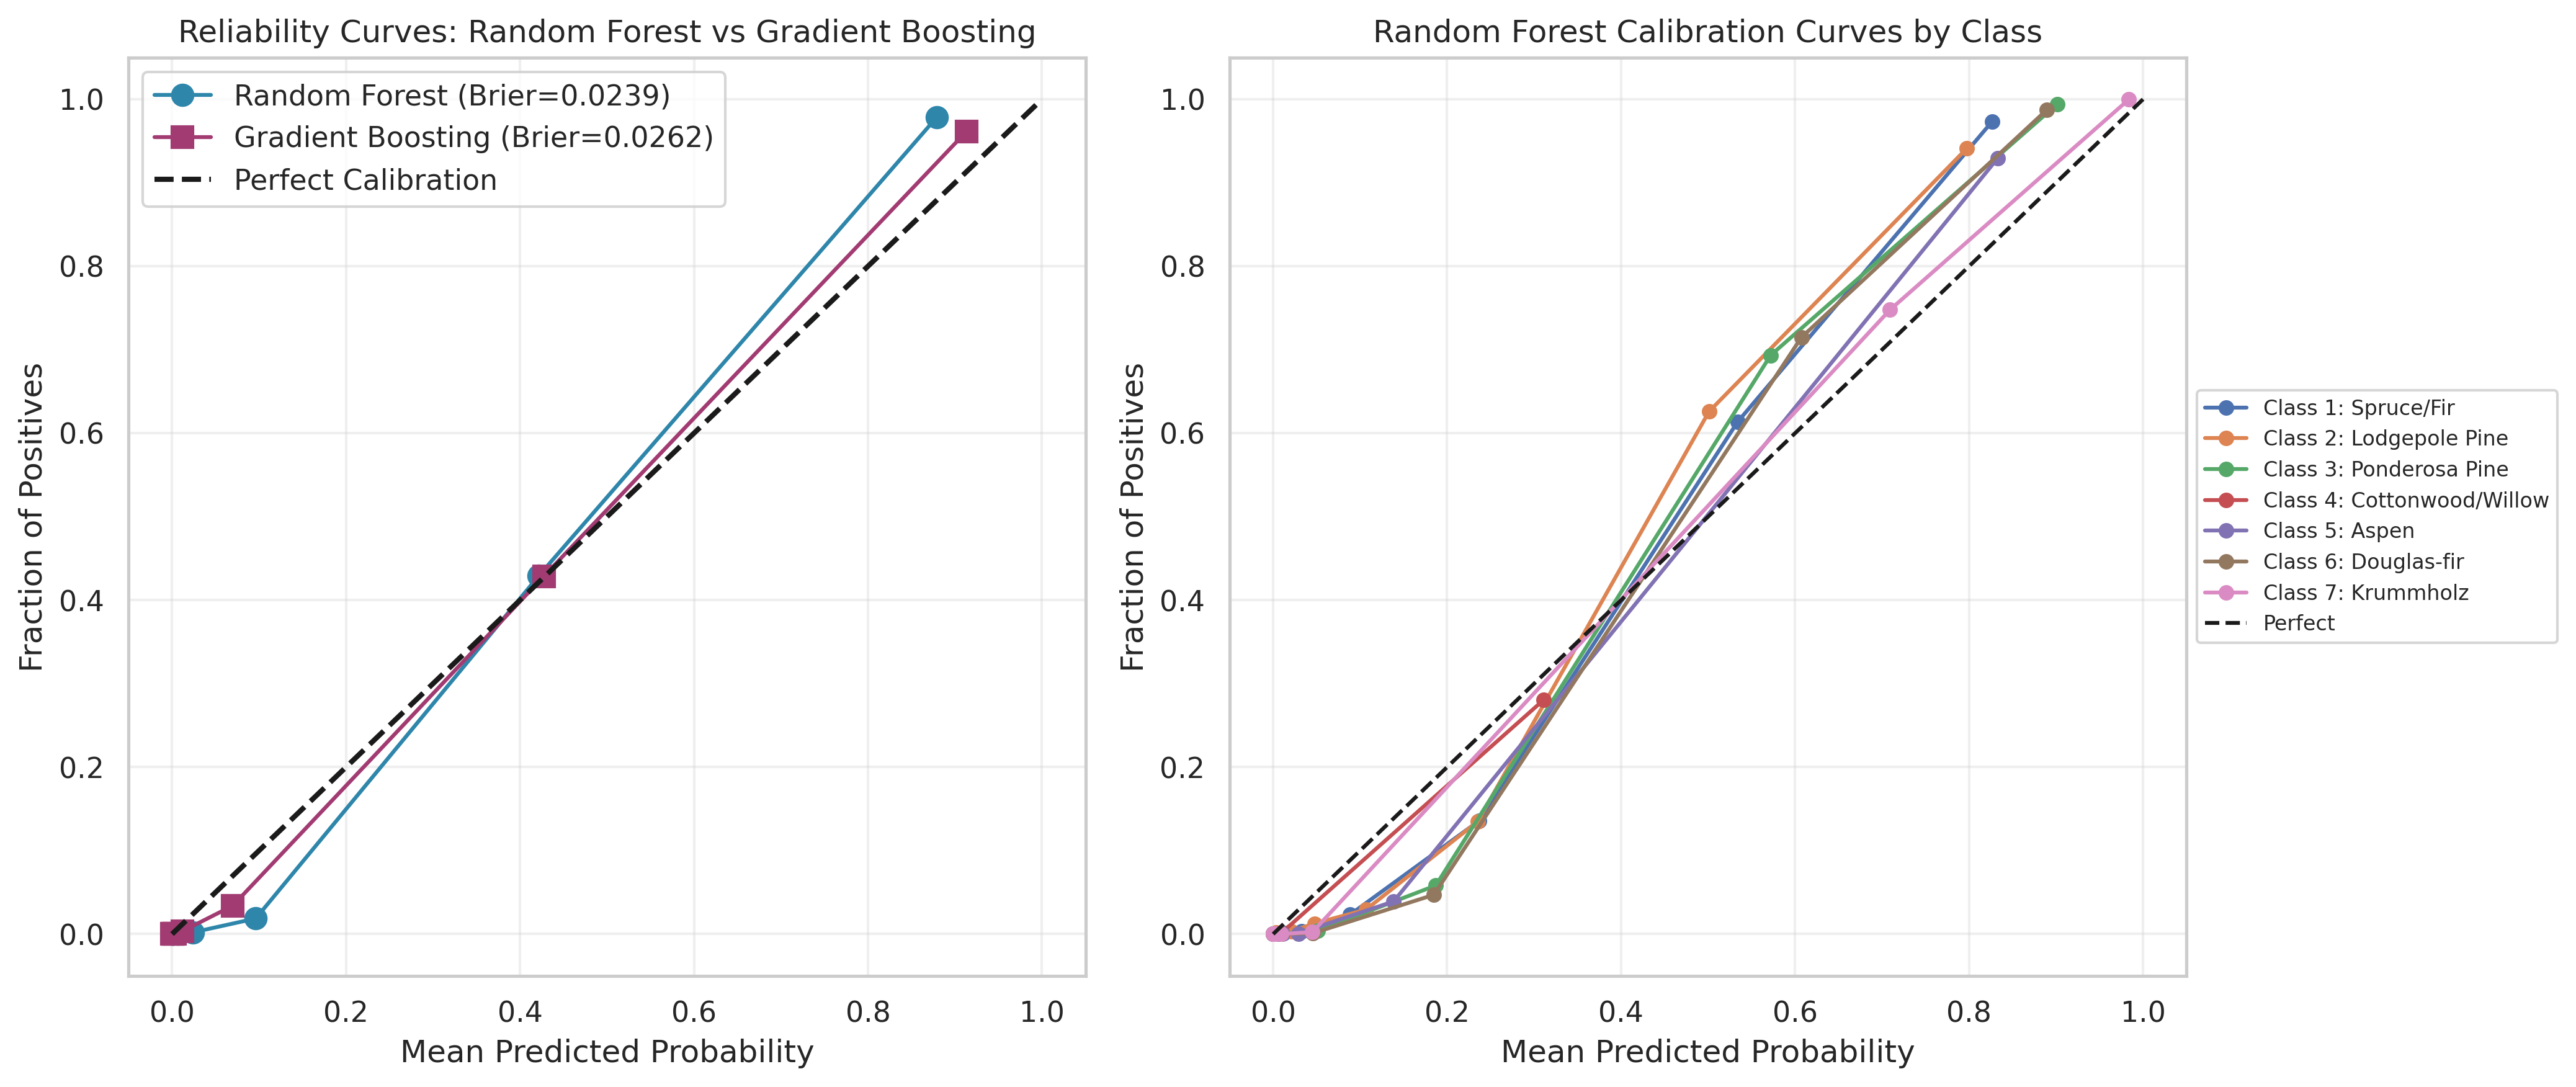
\includegraphics[width=\linewidth]{figures/calibration_reliability.png}\\[-0.4ex]
    \small (a) Reliability curves
  \end{minipage}\hfill
  \begin{minipage}{0.48\linewidth}
    \centering
    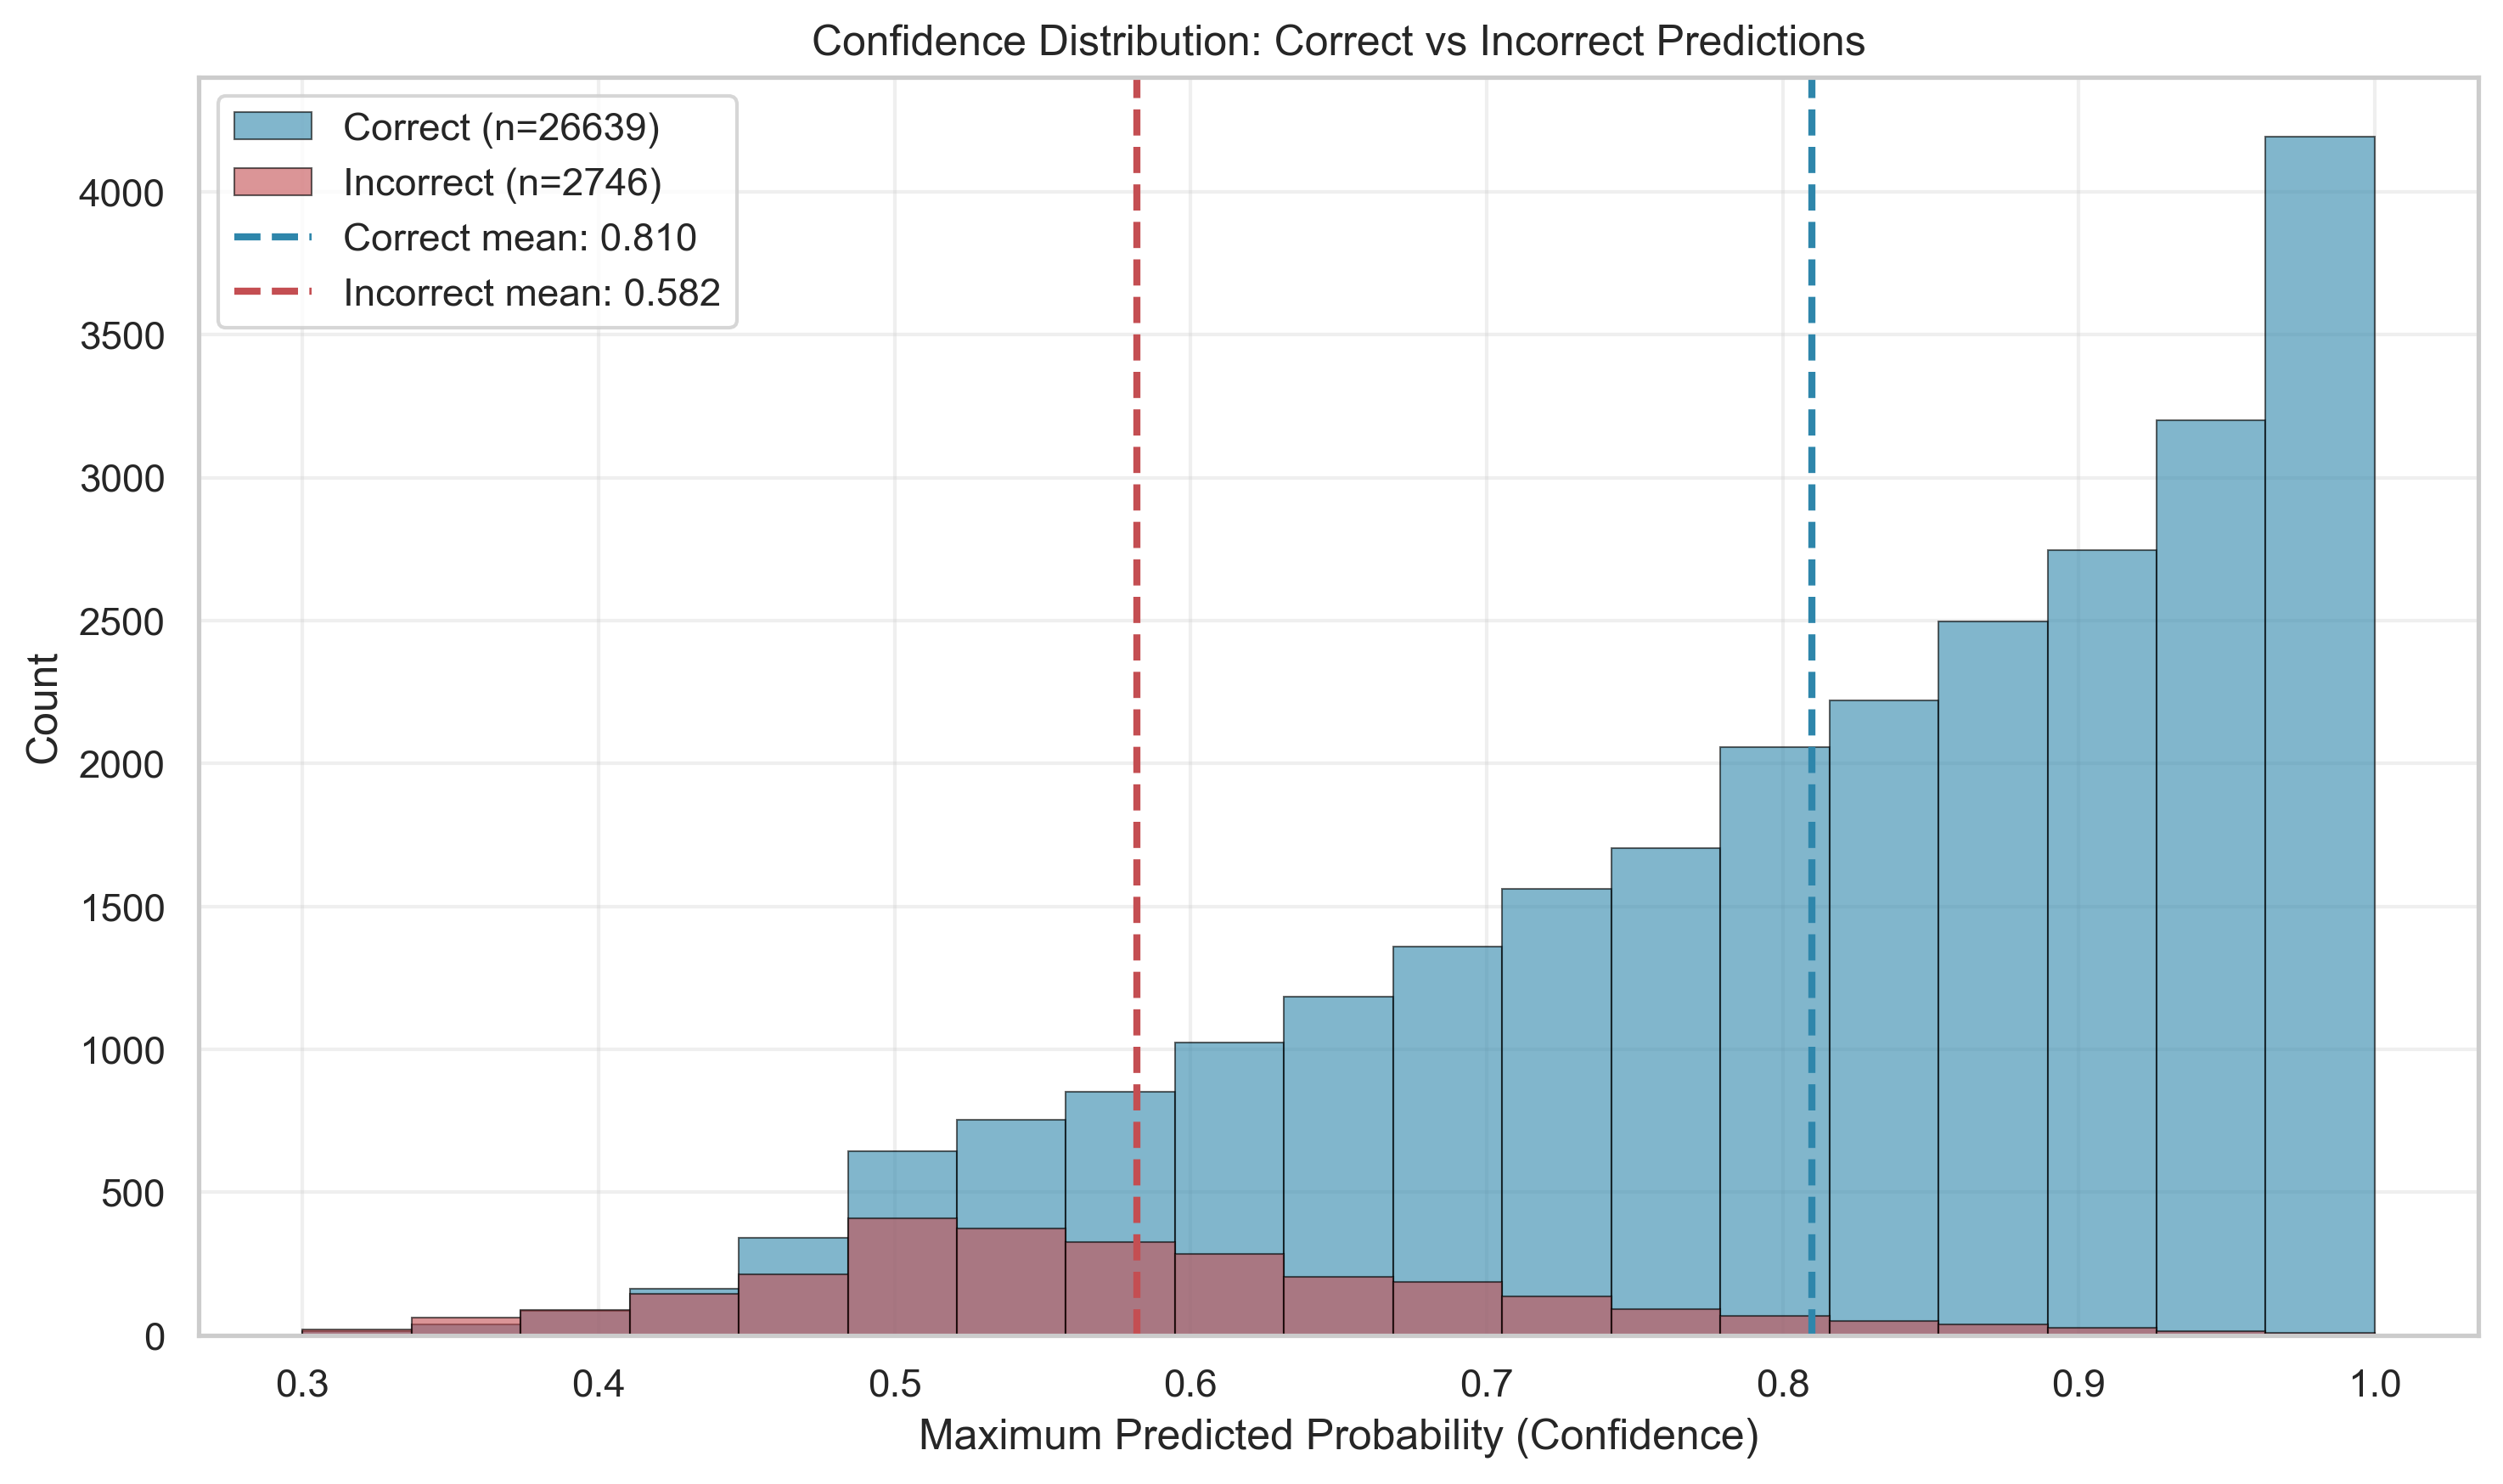
\includegraphics[width=\linewidth]{figures/error_confidence.png}\\[-0.4ex]
    \small (b) Confidence by correctness
  \end{minipage}
  \caption{Probability diagnostics. HistGradientBoosting is best calibrated, while Random Forest errors tend to receive substantially lower confidence than correct predictions.}
  \label{fig:calibration_errors}
\end{figure}

Performance also changes across terrain and classes. In Figure~\ref{fig:robustness}a, Random Forest accuracy rises from 0.863 in the most diverse elevation band to 0.958 in the highest; macro-F1 varies from 0.684 to 0.900. High-elevation Krummholz regions are therefore easier to distinguish than the mixed lower-elevation zones. Figure~\ref{fig:robustness}b gives the class-level view: Lodgepole Pine has the lowest recall (0.817), followed by Spruce/Fir (0.842), whereas Aspen, Douglas-fir, and Krummholz exceed 0.94 recall. These results show why both terrain-band metrics and macro scores are needed: a strong overall model can still have geographically and ecologically concentrated errors.

\begin{figure}[H]
  \centering
  \begin{minipage}{0.48\linewidth}
    \centering
    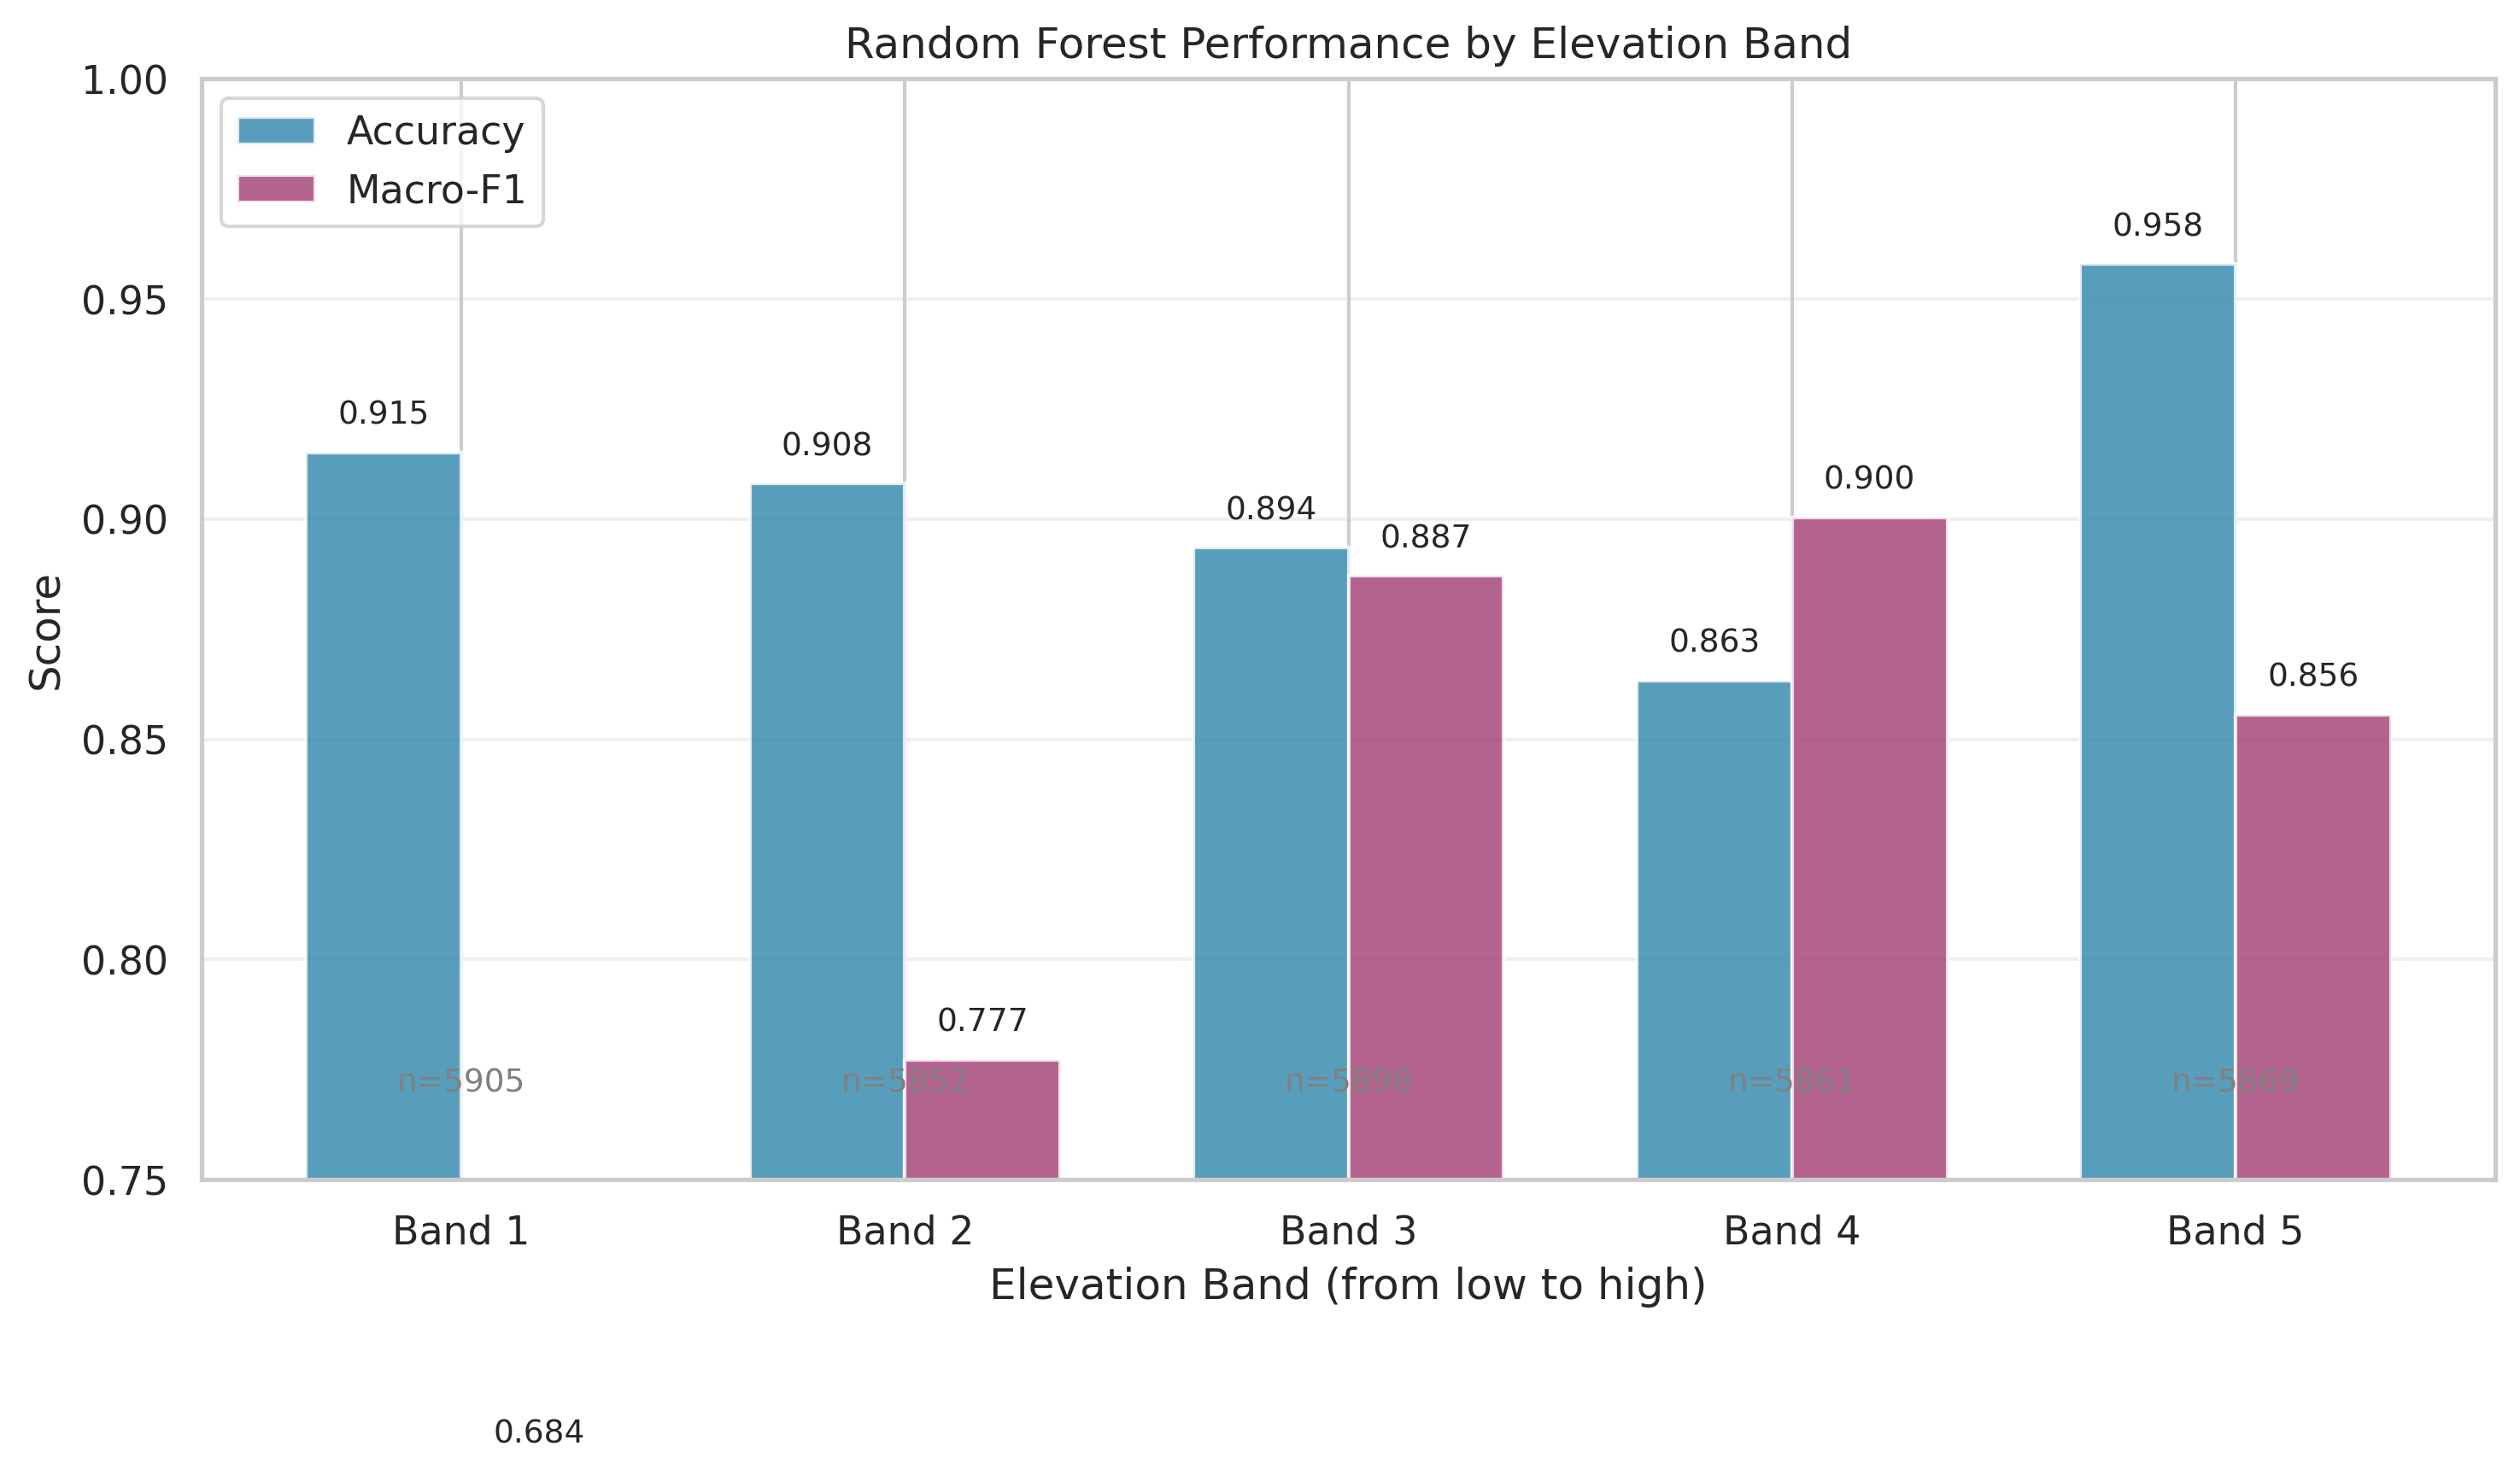
\includegraphics[width=\linewidth]{figures/elevation_band_accuracy.png}\\[-0.4ex]
    \small (a) Performance by elevation band
  \end{minipage}\hfill
  \begin{minipage}{0.48\linewidth}
    \centering
    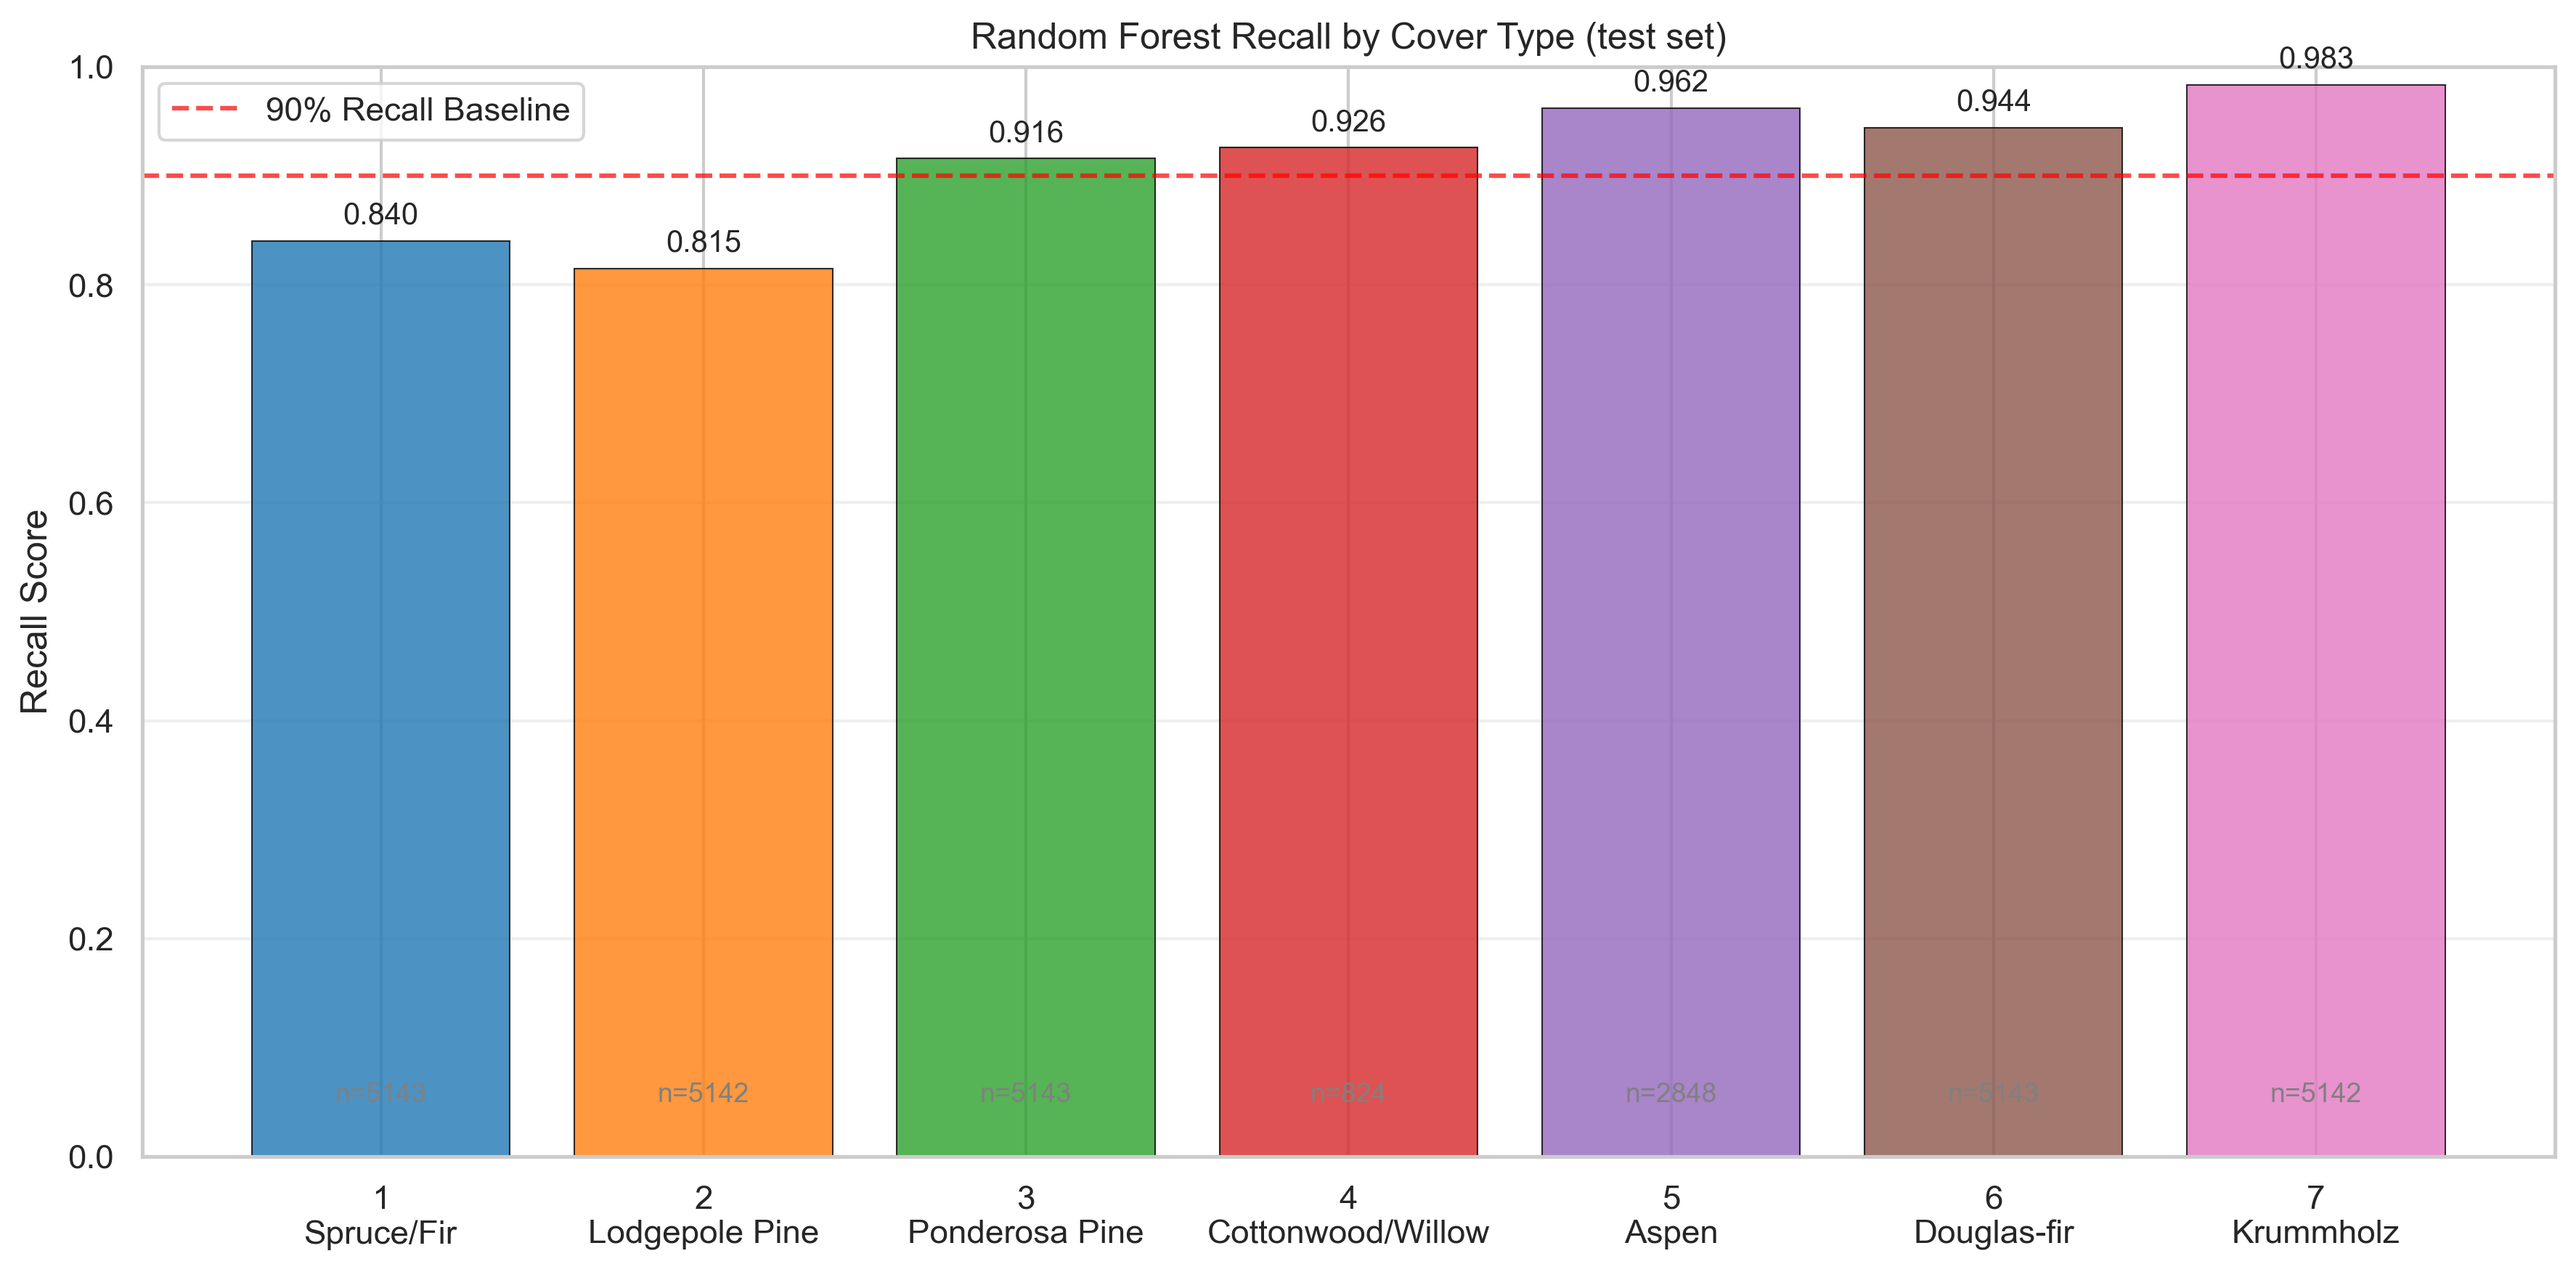
\includegraphics[width=\linewidth]{figures/class_recall_comparison.png}\\[-0.4ex]
    \small (b) Recall by cover type
  \end{minipage}
  \caption{Robustness of the selected Random Forest. Performance varies non-monotonically with elevation, while Lodgepole Pine and Spruce/Fir have the lowest per-class recall.}
  \label{fig:robustness}
\end{figure}

The four wilderness indicators identify geographic regions with different class composition.  Figure~\ref{fig:wilderness}a shows that Rawah is dominated by Lodgepole Pine, Neota and Comanche Peak by Krummholz, and Cache la Poudre by Ponderosa Pine; Comanche Peak has the highest normalized cover entropy (0.911).  Random Forest subgroup results (Figure~\ref{fig:wilderness}b) give accuracy/macro-F1 of 0.888/0.906 (Rawah), 0.924/0.866 (Neota), 0.915/0.910 (Comanche Peak), and 0.913/0.716 (Cache la Poudre).  Cache la Poudre has the most skewed class distribution and lowest macro-F1, consistent with its different dominant class and overlapping lower-elevation terrain.

\begin{figure}[H]
  \centering
  \begin{minipage}{0.48\linewidth}
    \centering
    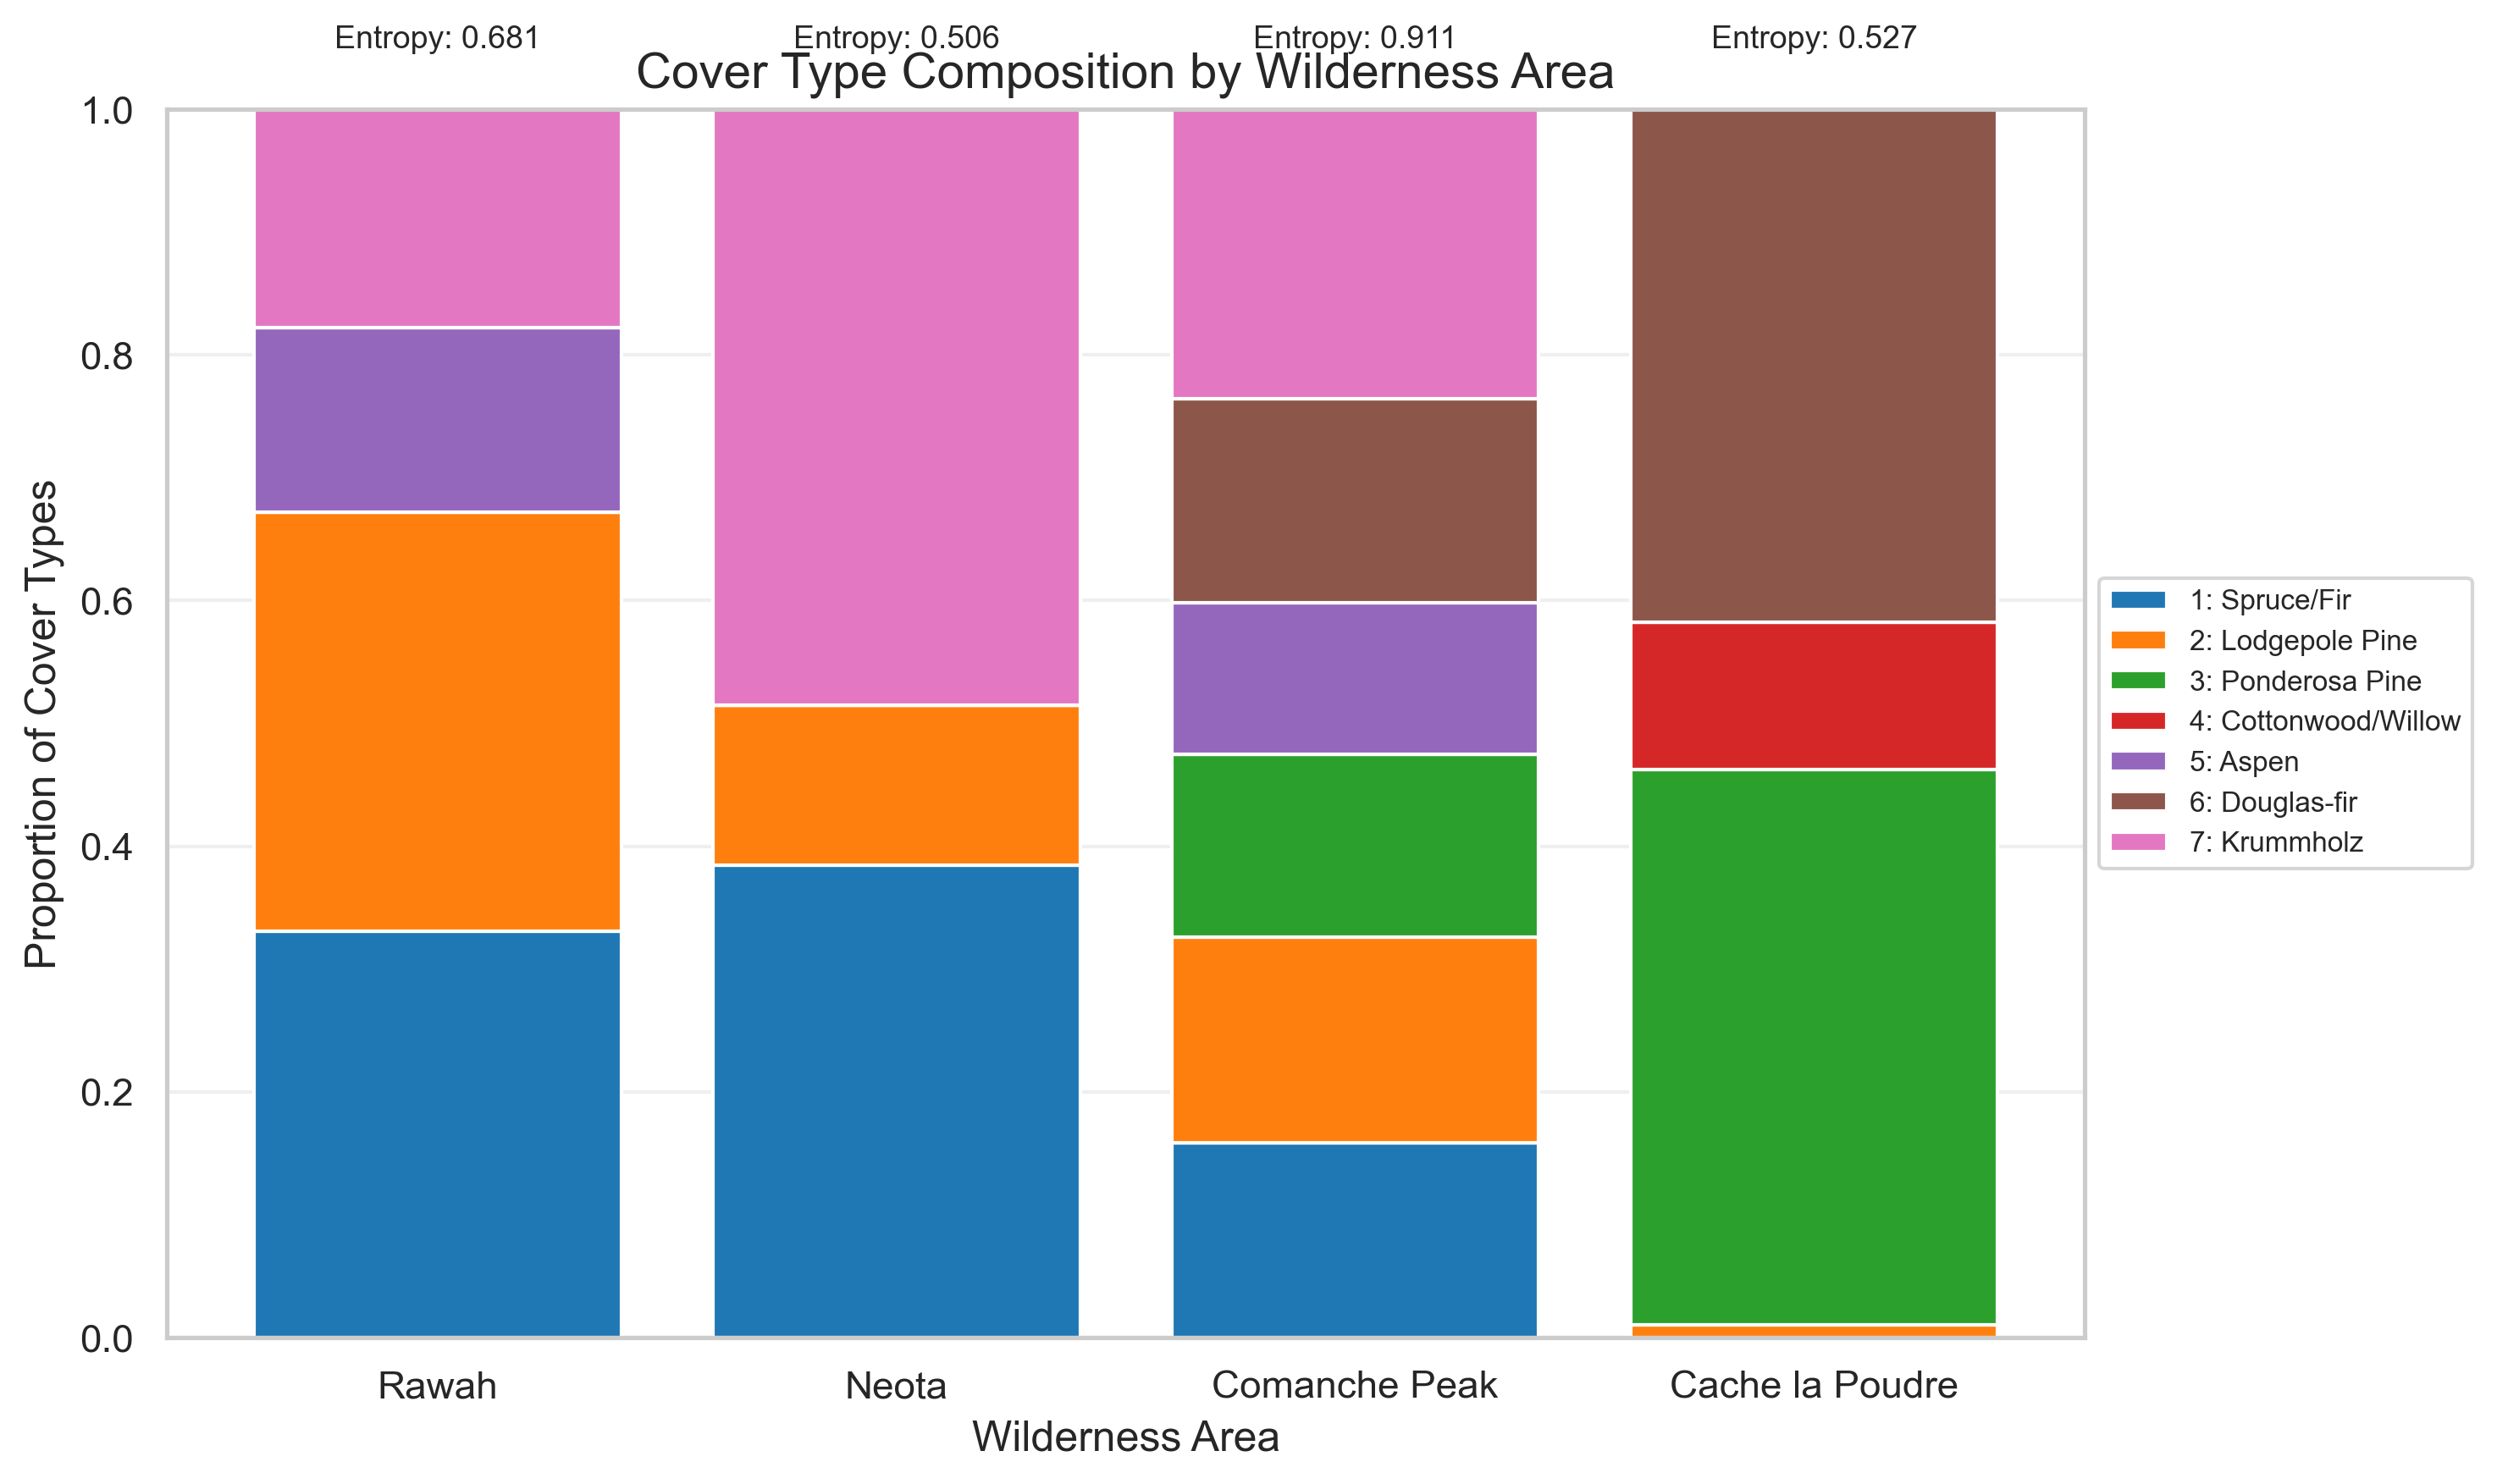
\includegraphics[width=\linewidth]{figures/wilderness_cover_distribution.png}\\[-0.4ex]
    \small (a) Cover composition by area
  \end{minipage}\hfill
  \begin{minipage}{0.48\linewidth}
    \centering
    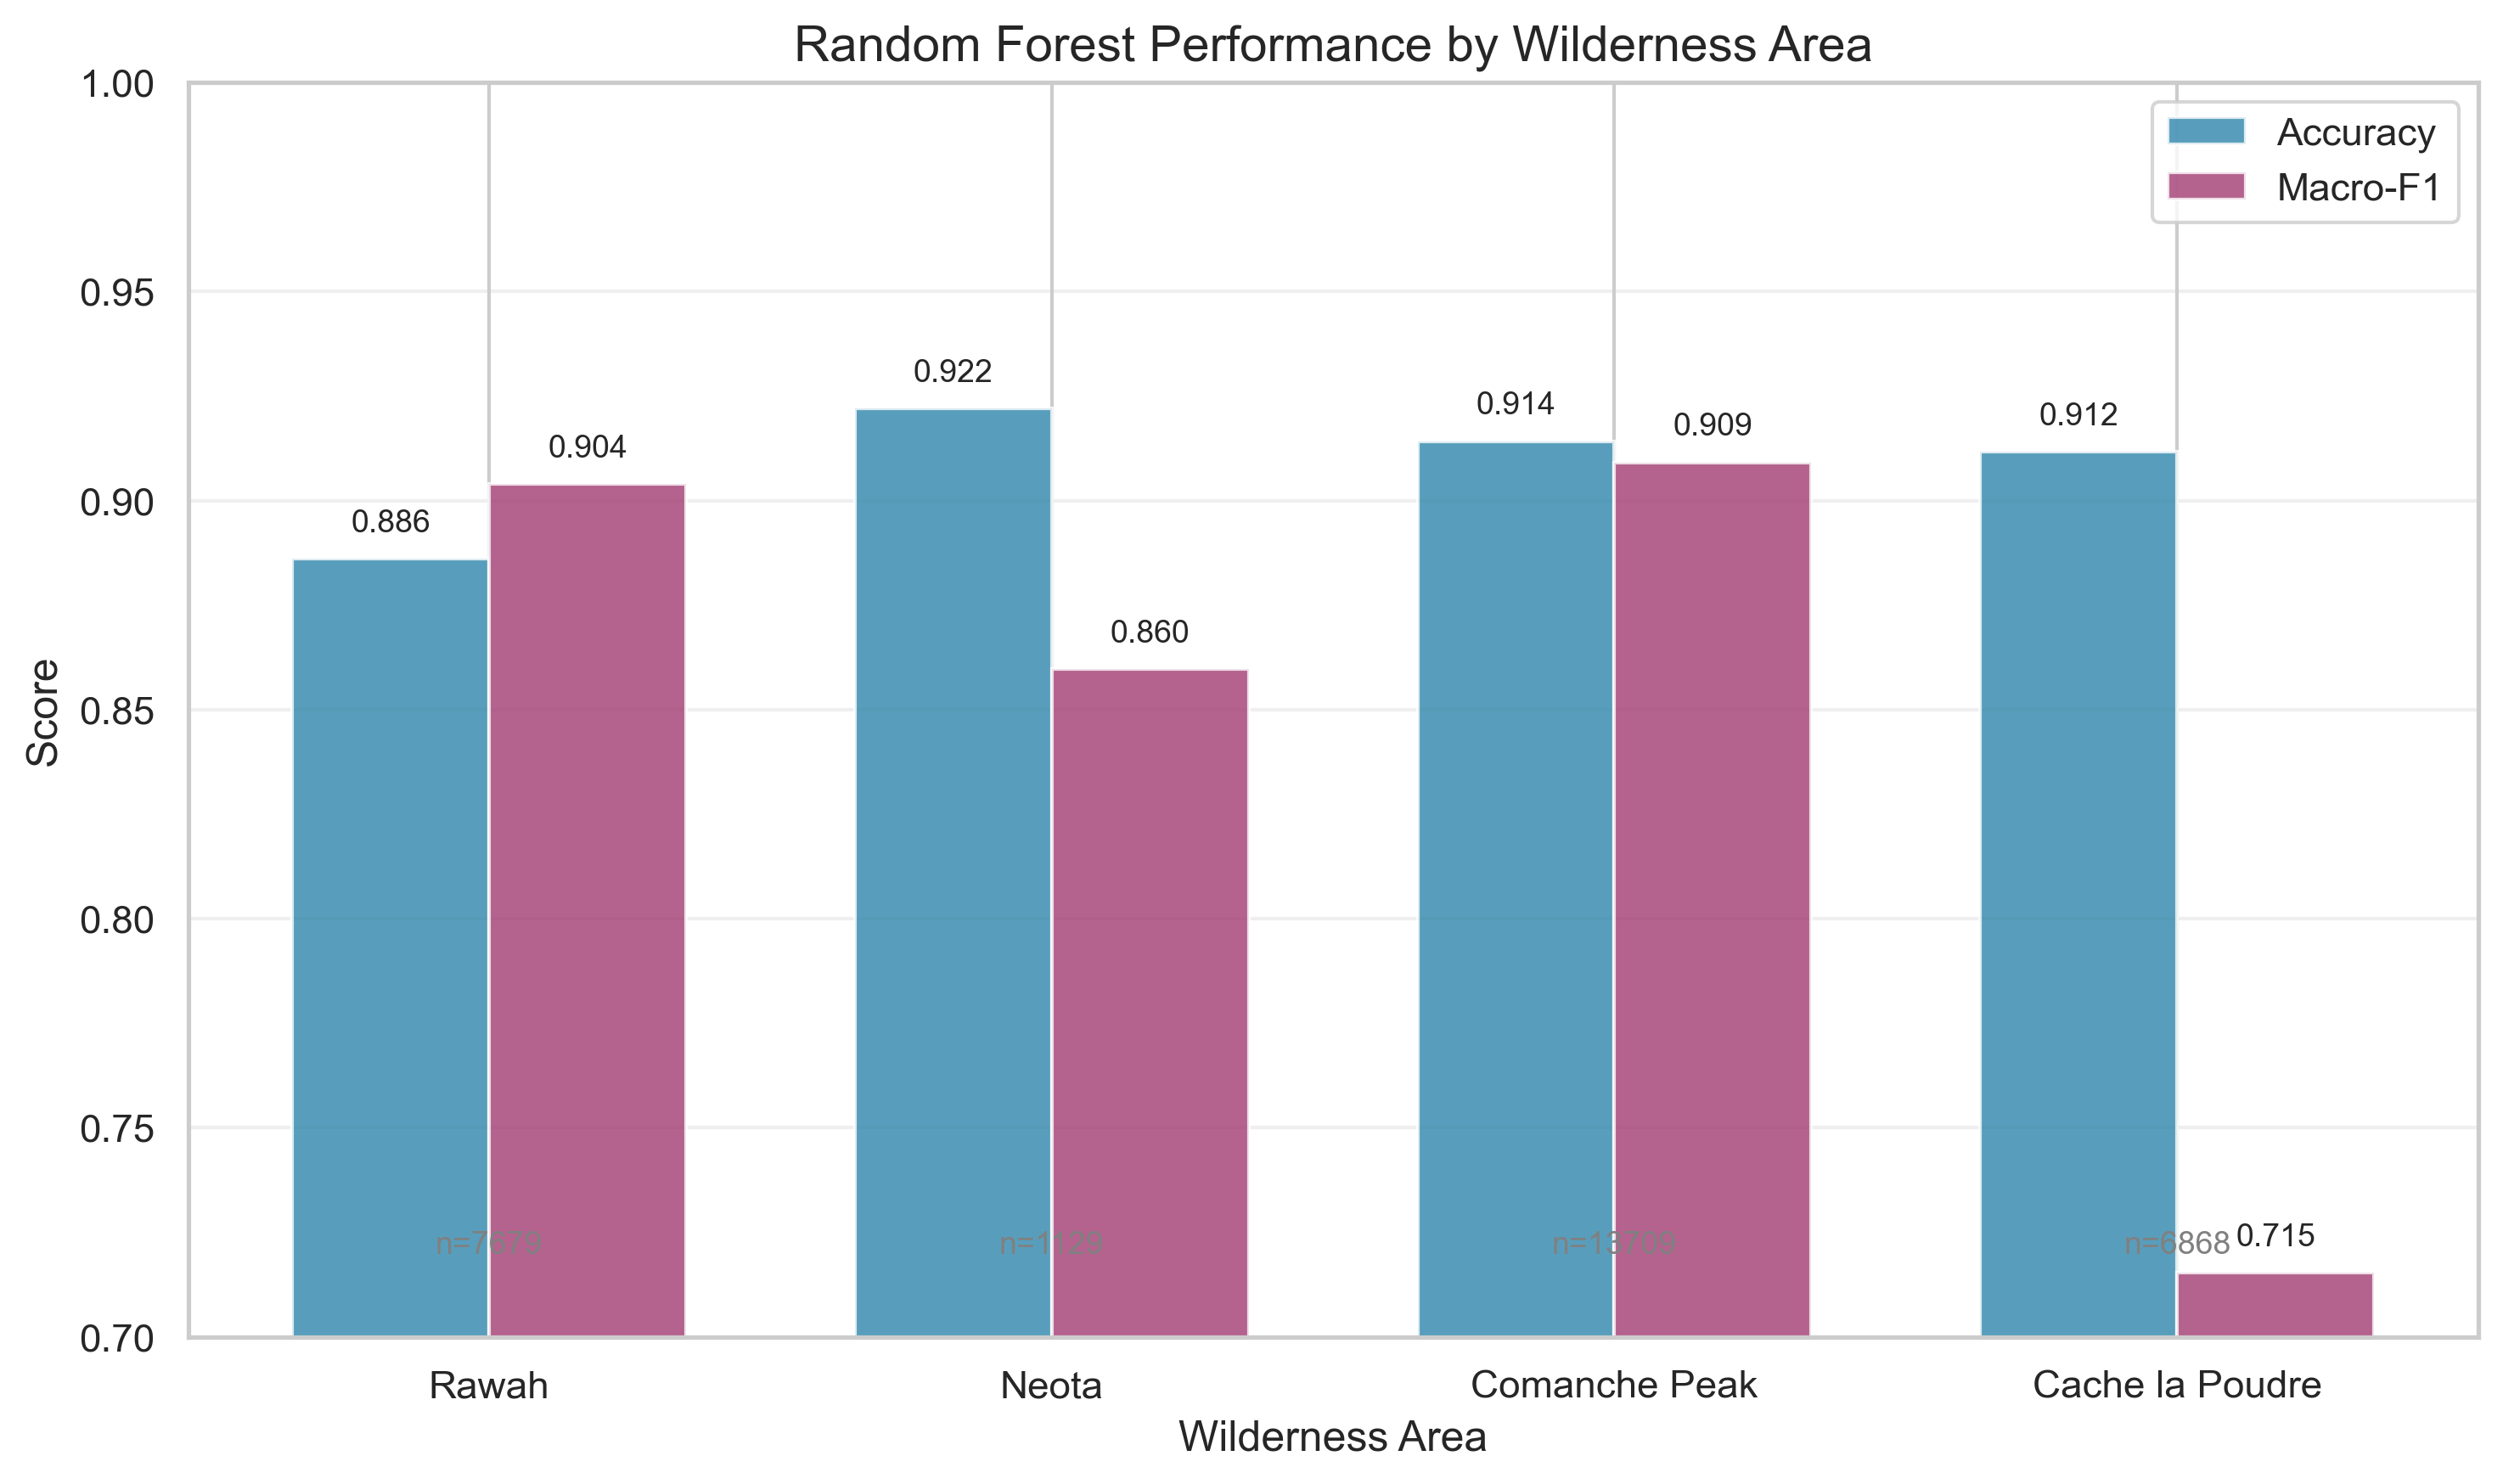
\includegraphics[width=\linewidth]{figures/wilderness_model_metrics.png}\\[-0.4ex]
    \small (b) Random Forest subgroup metrics
  \end{minipage}
  \caption{Wilderness-area extension. Geographic areas differ in both ecological composition and predictive difficulty, with Cache la Poudre producing the weakest results.}
  \label{fig:wilderness}
\end{figure}

\FloatBarrier
\section{Conclusion}

This project demonstrates that the Covertype labels are predictable even though they do not correspond to simple natural clusters. MiniBatchKMeans and Ward clustering achieve ARI of only 0.075 and 0.103.  Gower distance with complete linkage raises the post-hoc ARI to 0.245 ($k=4$), but this remains well below supervised accuracy (Random Forest 0.908). Random Forest produces the best held-out performance with 0.9076 accuracy, 0.9076 macro-F1, and 0.9923 macro AUC; the gap to HistGradientBoosting ($\Delta=0.0094$) is stable under bootstrap but practically negligible. Elevation dominates feature importance; terrain alone achieves 0.874 F1, while polynomial features yield zero gain for logistic regression. Remaining errors are structured: Lodgepole Pine and Spruce/Fir have the lowest recall, the most diverse elevation band is hardest, and Cache la Poudre is the weakest wilderness area. Grid search on a 30k subset degrades performance; Bayesian optimization recovers baseline — confirming the bottleneck is search strategy, not subset size. The modeling sample covers $\approx$17\% of the full dataset; full-data gradient boosting reaches 0.95--0.96 accuracy in the literature \cite{kaggle}. The most reliable deployment combines macro metrics, calibration checks, and subgroup validation.

{\footnotesize
\begin{thebibliography}{99}
  \bibitem{blackard1998comparison}
  J.~A. Blackard, ``Comparison of neural networks and discriminant analysis in predicting forest cover types,'' Ph.D. dissertation, Colorado State University, 1998.

  \bibitem{blackard1999comparative}
  J.~A. Blackard and D.~J. Dean, ``Comparative accuracies of artificial neural networks and discriminant analysis in predicting forest cover types from cartographic variables,'' \textit{Computers and Electronics in Agriculture}, vol.~24, no.~3, pp.~131--151, 1999.

  \bibitem{uci}
  UCI Machine Learning Repository, ``Covertype,'' \url{https://archive.ics.uci.edu/dataset/31/covertype}.

  \bibitem{tsne}
  L.~van der Maaten and G.~Hinton, ``Visualizing data using t-SNE,'' \textit{Journal of Machine Learning Research}, vol.~9, pp.~2579--2605, 2008.

  \bibitem{sklearn}
  F.~Pedregosa et al., ``Scikit-learn: Machine learning in Python,'' \textit{Journal of Machine Learning Research}, vol.~12, pp.~2825--2830, 2011.

  \bibitem{kaggle}
  Kaggle, ``Forest Cover Type Prediction,'' \url{https://www.kaggle.com/c/forest-cover-type-prediction}.

  \bibitem{optuna}
  T.~Akiba, S.~Sano, T.~Yanase, T.~Ohta, and M.~Koyama, ``Optuna: A Next-generation Hyperparameter Optimization Framework,'' in \textit{Proceedings of the 25th ACM SIGKDD}, 2019, pp.~2623--2631.

  \bibitem{probst2019}
  P.~Probst, A.-L.~Boulesteix, and B.~Bischl, ``Tunability: Importance of Hyperparameters of Machine Learning Algorithms,'' \textit{Journal of Machine Learning Research}, vol.~20, no.~53, pp.~1--32, 2019.
\end{thebibliography}
}

\section*{Credit and GenAI Use}

{\small
\textbf{Group member contributions.}
\begin{itemize}[leftmargin=*,itemsep=1pt,topsep=3pt]
  \item \textbf{Zeyun DU}: data preprocessing, visualization, clustering, model evaluation, code implementation, and figure generation.
  \item \textbf{Zixiang QIN}: feature importance, model selection, calibration, robustness, and subgroup diagnostics.
  \item \textbf{Chunfeng GAO}: computational optimization, report preparation, result checking, and final editing.
\end{itemize}

\textbf{GenAI Tools Usage:}
\begin{itemize}[leftmargin=*,itemsep=1pt,topsep=3pt]
    \item OpenAI Codex was used to draft, refactor, and validate parts of the analysis workflow and report (approximately 10\% of the combined support effort).
    \item Doubao was used to polish and refine the report writing (approximately 10\% of the report-writing support effort).
    \item DeepSeek and Claude were used for overall review, statistical rigor checks, and methodological critique of the analysis and report (approximately 10\% of the revision support effort).
\end{itemize}

\end{document}
